\documentclass[draft]{agujournal2019}

\newcommand{\todo}[1]{\textcolor{red}{\textbf{(#1)}}}

\usepackage{amsmath}

% LTeX: language=en-US

\linenumbers
\journalname{Journal of Advances in Modeling Earth Systems (JAMES)}

\begin{document}

\title{Responses to Humidity and Temperature Perturbations in High-Resolution Simulations of Convection}

\authors{Timothy H. Raupach\affil{1,2}, Chimene L. Daleu\affil{3}, Robert S.
Plant\affil{3}, Steven C. Sherwood\affil{1,2}, and Yi-Ling Hwong\affil{4}}

\affiliation{1}{Climate Change Research Centre, University of New South Wales, Sydney, Australia}
\affiliation{2}{ARC Centre of Excellence for Climate Extremes}
\affiliation{3}{Department of Meteorology, University of Reading, Reading, United Kingdom}
\affiliation{4}{Institute of Science and Technology Austria, Vienna, Austria}

\correspondingauthor{Timothy H. Raupach}{timothy.h.raupach@gmail.com}

\begin{keypoints}
    \item For the two models examined, accurate simulation of
    convectively-coupled dynamics requires a grid spacing of lower than $\sim$1
    km.
    \item The linear responses of LES models with sufficient resolution in these
    idealised tests could reasonably be used as ground truth for Global Climate
    Model scheme testing.
\end{keypoints}

\justifying
\begin{abstract}
\todo{Abstract\ldots}
\end{abstract}

\section*{Plain Language Summary}
\todo{Plain language summary\ldots}

\section{Introduction}

Global and regional climate models (respectively GCMs and RCMs) must take
convection into account because of its important atmospheric effects
\cite{Manabe_JAS_1964, Wallace_2006}. However, models often use horizontal grid
spacings that are much larger than the horizontal scale of convection, meaning
that they are unable to resolve individual convective cells. In this case, the
model must account for the effects of convection -- such as its heating effect
or the rain it may produce -- by parameterizing the sub-grid convection that it
can not explicitly resolve. Such parameterization methods are called convection
schemes. 

Many convection schemes have been produced, each with different strengths,
weaknesses, and assumptions \cite<e.g.>{Arakawa_JC_2004, Rio_CCCR_2019,
Lin_AO_2022}. Such are the differences between these schemes, and so high is the
sensitivity of models to convective cloud physics \cite<e.g.>{Emanuel_JAS_1999},
that convection parameterization is a leading source of uncertainty in model
outputs \cite<e.g.>{Hwong_JAMES_2021}. It is difficult to compare convection
schemes, since traditional methods in which simulated outputs are compared with
observations \cite<e.g.>{Grell_ACP_2014, Kwon_MWR_2017, Zhang_JC_2017,
Zhang_MWR_2011} are limited by observation selection and accuracy
\cite{Hwong_JAMES_2021}.

The mathematical framework proposed by \citeA{Kuang_JAS_2010} uses a linear
tangent model to approximate the feedback of small-scale processes on the
large-scale environment, effectively playing the role of a (linear) convective
scheme trained on a large cloud-resolving model (CRM) dataset, such that

\begin{equation} 
\frac{\partial {\bf X}}{\partial t} = {\bf MX}
\end{equation}

where the partial time derivative represents the feedback on the column state
variable {\bf X}, and {\bf M} is a matrix obtained from perturbed runs of a
cloud-resolving model. In this method, the responses of the model (and thus the
convection scheme) are examined in idealized simulations under different small
perturbations to the humidity and temperature tendencies. The idea is that
although there are many non-linear processes in convection, the statistics of
the cumulus ensemble as a whole can be partly described by smooth linear
functions that describe how the ensemble reacts to small changes in its
large-scale environment. \citeA{Kuang_JAS_2010} provided evidence that these
linear responses were sufficient to capture the dynamics of convectively-coupled
waves, which evolve slowly compared to typical convective response times and
have relatively small amplitudes. Even if a linear approximation is inadequate
for fully describing convection for more general purposes, it can be a useful
first-order characterization.

To this end, the linear response framework was applied to single column models
(SCMs) by \citeA{Herman_JAMES_2013} specifically for the purpose of testing two
convection schemes against the equivalent tangent linear model constructed from
a CRM reference. \citeA{Hwong_JAMES_2021} used the framework to evaluate
convection, planetary boundary layer, and microphysics schemes' responses to
perturbations in SCMs. They showed that the results isolate the impact of the
convection scheme in at least the tested SCMs, and examined many other schemes
in common use. The technique allows for efficient comparison of different model
setups, and identified a wide range of responses among current schemes, thus
showing the potential of this test. However, the study did not attempt to answer
the question of which setup was the most accurate. To answer this question we
need a "truth" response, which is not available from observations. A study of
the linear responses of a model that uses the least possible parameterization is
therefore required, along with robustness tests. \citeA{Kuang_JAS_2010}
evaluated his linear responses using rather coarse resolution (2 km)  runs of
the System for Atmospheric Modelling \cite<SAM, e.g.>{Khairoutdinov_JAS_2003},
and in a relatively small domain (128 km square). This resolution would not be
considered large-eddy resolving by today's standards, and the experiment has not
been repeated in any other cloud-resolving model.

In this study, we repeated the above perturbation experiments with two different
models across a range of CRM and large eddy simulation (LES) resolutions,
seeking to produce benchmark test results. This also enabled us to test the
conclusion of \citeA{Hwong_JAMES_2021} that the results are not sensitive to the
treatment of the planetary boundary layer (PBL), for configurations in which
convection is resolved explicitly and the PBL dynamics interact more directly
with it. The key question is whether the linear responses are robust, or
sensitive to decisions made in high-resolution modelling such as the grid
length, model dynamical core, or treatment of microphysics or eddy mixing; in
particular, can we establish a reference ``truth'' that is less uncertain than
the variations between convection schemes themselves? A related question is
whether the response is dominated by the modelled convection itself, or whether
it might be sensitive to the specification of surface properties in an idealized
modelling setting. A third question addressed here, which is becoming more
relevant as we enter an age of global CRMs, is what grid resolution they would
need to properly represent convective-scale feedbacks on large scale flows,
arguably the key benefit of global CRMs, and how sensitive the feedback might be
to parameterizations remaining in those models or to the numerics or other
details of the CRM. In summary, how should we judge differences between model
schemes as reported in \citeA{Hwong_JAMES_2021} using LES or CRM models?

\section{Methods}
\label{sec:methods}

We used two numerical models in this work: the Advanced Research (AR) version of
the Weather Research and Forecasting (WRF) model, version 4.1.4
\cite{Skamarock_2019}, and the Met Office/NERC Cloud Model
\cite<MONC,>{Brown_2020}.

\subsection{Common Model Settings}

Both models were used to simulate convection at high resolution over a water
surface with periodic boundary conditions. The models used a constant sea
surface temperature (SST) of 301.15 K. This value is a little different from
that used in \citeA{Kuang_JAS_2010} but matches \citeA{Hwong_JAMES_2021}. We
used idealized radiation as in \citeA{Kuang_JAS_2010}, \citeA{Herman_JAMES_2013}
and \citeA{Hwong_JAMES_2021}. Following \citeA{Herman_JAMES_2013}, the radiative
cooling tendency was $\partial \theta_{rad} / \partial t = \theta_t/\Pi$ K
day$^{-1}$, where $\Pi$ is the Exner function that converts temperature to
potential temperature, and $\theta_t$ is a temperature tendency set as
\todo{THR: I've updated the linear part to reflect WRF, does it match the MONC
setting?}

\begin{align}
 \theta_t = \begin{cases}
    -1.5\; \textrm{K day}^{-1} & \textrm{if}\, p \geq 200\; \textrm{hPa}, \\
    0\; \textrm{K day}^{-1} & \textrm{if}\, p \leq 100\; \textrm{hPa}, \\
    -\frac{1.5 (p-100)}{100}\; \textrm{K day}^{-1} & \textrm{if}\, 
    100 < p < 200\; \textrm{hPa}. \\
 \end{cases}
\end{align}

Our treatment of surface fluxes and winds also follows that of
\citeA{Hwong_JAMES_2021}, which differed slightly from that of
\citeA{Kuang_JAS_2010}. First, we used idealized evaporation as in
\citeA{Chua_GRL_2019}, with minor differences. We used a constant surface wind
speed of $W_s = 5$ m s$^{-1}$, following \citeA{Hwong_JAMES_2021} who used the
same approach with a fixed value of 0.001 for the surface exchange coefficient.
While the wind speed here and in \citeA{Hwong_JAMES_2021} was slightly different
from that of \citeA{Kuang_JAS_2010}, the important quantity is the product of
the wind with the surface exchange coefficient, and the exchange coefficient
value in \citeA{Kuang_JAS_2010} was not stated. Here we used a fixed value of
0.005 for this quantity. Level-mean horizontal winds were relaxed to $u = 0$ m
s$^{-1}$ and $v = 5$ m s$^{-1}$, where $u$ and $v$ are orthogonal wind
components, with a three-hour relaxation time.

\todo{THR: For equations 3, 4, and 5 and the associated descriptions, please
could you confirm they are correct for MONC, Chimene or Bob?}

We used idealized evaporation as in \citeA{Chua_GRL_2019} and
\citeA{Hwong_JAMES_2021}, with a fixed surface wind speed and the drag
coefficient assumed to be 0.001. Then surface heat flux (SH) was calculated
using modified Equation 1 from \citeA{Chua_GRL_2019}, such that

\begin{equation}
\textrm{SH} = 0.001 \rho_a W_s c_p (T_s - T_a),
\end{equation}

\noindent where $\rho_a$ (kg m$^{-3}$) is the near surface air density, $T_s$
(K) is surface temperature (we use SST), and $T_a$ (K) is the near-surface air
temperature. We used 

\begin{equation}
T_a = T_l \left(\frac{p_s}{p_l}\right)^{\frac{R_d}{c_p}},
\end{equation}

\noindent where $T_l$ (K) is the temperature at the first model level above the
surface, $p_s$ (hPa) is surface pressure, $p_l$ (hPa) is pressure at the first
model level, $c_p$ (J kg$^{-1}$ K$^{-1}$) is the specific heat capacity of dry
air at constant pressure, and $R_d$ (J kg$^{-1}$ K$^{-1}$) is the gas constant
for dry air. Latent heat flux (LH) was calculated using modified Equation 2 from
\citeA{Chua_GRL_2019}, such that

\begin{equation}
\textrm{LH} = 0.001 \rho_a W_s L (q_{sat} - q_a),
\label{eq:LH}
\end{equation}

\noindent where $L$ is the latent heat of vaporization of water, $q_{sat}$ is
the saturated water vapor mixing ratio at $T_s$ and $q_a$ is the water vapor
mixing ratio at the lowest model level. 

Because the pressure levels in the WRF model were not exactly at the points
around which we want to perturb, we adapted the form of perturbations used by
\citeA{Herman_JAMES_2013} so that only the Gaussian portion of the perturbation
function was used, and instead of selecting a level $k$ a pressure $p_p$ (hPa)
around which to perturb was selected. The perturbation function used in the WRF
simulations for the $i$th model level was

\begin{equation}
\frac{d}{dt} \chi = A \exp\left[ - \left( \frac{p_p - p_i}{75 \textrm{hPa}}\right)^2 \right],
\end{equation}

\noindent where $p_p$ (hPa) is the chosen perturbation pressure and $p_i$ is the
pressure at level $i$, $\chi$ is the variable subject to the extra forcing, and
$A$ is the amplitude of forcing. 

Following \citeA{Kuang_JAS_2010}, for each resolution, the models were run until
they reached radiative convective equilibrium (RCE) at time $t_1$. After RCE was
reached, small perturbations in the imposed temperature or moisture forcings
were introduced, while a control was continued from $t_1$ with no perturbations.
The simulations were all allowed to again reach an equilibrium at time $t_2$. To
construct RCE mean profiles, we first calculated spatial means of each output
variable studied per interpolated model pressure level, per time step, then
calculated the temporal average of these mean profiles over the RCE period.

For a time block after $t_2$, domain-mean profiles from the control runs were
subtracted from the domain-mean atmospheric profiles for the perturbed runs to
examine the differences induced by the forcing perturbations. In the following
two sections we examine model-specific aspects of the setups for WRF and MONC,
respectively.

\subsection{WRF}

WRF was run on a 20 $\times$ 20 km$^2$ domain for horizontal grid spacings of 4
km, 1 km and 100 m. The runs at 4 km and 1 km grid resolution used 74 grid
levels in the vertical while the run at 100 m grid spacing used 370 levels. The
parameterizations used are summarized in Table \ref{tab:WRF_schemes}. The model
time step was set to 6 s for 4 km and 1 km grid spacing and 1 s for 100 m grid
spacing, and outputs were recorded hourly for the 1 km and 4 km cases, and at 2
hour resolution for the 100 m cases. For the runs with 1 km and 4 km grid
spacing, the models were initialized using a Radiative-Convective Equilibrium
Model Intercomparison Project (RCEMIP) profile \cite{Wing_GMD_2018}. For the
runs at 100 m grid spacing, the model was initialized using the mean RCE model
state from the 1 km control run, so that the LES runs started near RCE to reduce
computation time. Temperature and water vapor mixing ratio in the stratosphere
were relaxed to the initial profile values to avoid model drift, as suggested by
\citeA{Herman_JAMES_2013}. Relaxation was applied above 160 hPa with the inverse
relaxation constant increasing linearly from $1/\tau = 0$ day$^{-1}$ at 160 hPa
to $1/\tau = 0.5$ day$^{-1}$ at and above 100 hPa \cite{Herman_JAMES_2013}. Full
diffusion was used at all resolutions; at 4 km and 1 km resolutions, horizontal
diffusion was diagnosed from deformation and vertical diffusion was assumed done
by the planetary boundary layer scheme (\texttt{km\_opt = 4}) while the
simulations at 100 m used a prognostic equation (\texttt{km\_opt = 2}) for
turbulent kinetic energy \cite{Skamarock_2019}. For $q_{sat}$ we use WRF's
``ground saturated mixing ratio'', and in Equation \ref{eq:LH} we used the
near-surface air density value produced by WRF (around 1.16 kg m$^{-3}$) rather
than the value of 1 km m$^{-3}$ assumed by \citeA{Chua_GRL_2019}.

\begin{table}[t]
    \caption{Parameterizations used in the WRF simulations. These schemes were
     used for all resolutions, except that the boundary layer scheme was enabled
     only for the 4 km and 1 km simulations. No convection parameterization was
     used.}
    \label{tab:WRF_schemes}
    \centering
    \begin{tabular}{lll}
    \hline
    \textbf{Parameterization} & \textbf{Scheme} & \textbf{Reference} \\
    \hline
    Microphysics & Thompson 2-moment & \citeA{Thompson_MWR_2008} \\
    Boundary layer & YSU & \citeA{Hong_MWR_2006} \\
    Surface layer & Revised MM5 & \citeA{Jimenez_MWR_2012} \\
    \hline
    % \multicolumn{2}{l}{$^{a}$Footnote text here.}
    \end{tabular}
\end{table}

\subsection{MONC}

MONC was run on a 64 $\times$ 64 km$^2$ domain for grid spacings of 1 km, 500 m,
and 250 m. The MONC setup was similar to that used in \citeA{Daleu_QJRMS_2023}:
the domain height was 20 km, with 85 levels on a stretched grid so there were
more levels near the surface, and a Newtonian damping layer above 16 km. The 3D
Smagorinsky scheme \cite{Smag63,Lilly67} was used to calculate subgrid turbulent
eddy fluxes, and the Cloud AeroSol Interactive Microphysics \cite<CASIM,
see>{field23} scheme represented cloud processes. The model time step is
variable in MONC and ranged between 1 and 2 seconds. Perturbations were made
using a combination of the delta and Gaussian functions, as in Equation~4 of
\citeA{Herman_JAMES_2013}. For pressure levels less than 160 hPa, temperature
and moisture fields were relaxed to the values of a previous RCE run, following
\cite{Herman_JAMES_2013}.

\subsection{Perturbations to Temperature and Humidity}

Constant perturbations were applied to potential temperature or water vapor
tendencies at given model levels. Given computational constraints, not all
perturbations were applied for all of the resolutions.  Table
\ref{tab:pert_runs} shows which perturbations were applied for which grid
spacings. We used the WRF results of \citeA{Hwong_JAMES_2021} to select two
levels on which perturbations provided the most information about perturbations
across a range of other levels (not shown here). The two ``most representative''
levels were a low (850 hPa) and a high (412 hPa) perturbation level. Within
MONC, it was convenient to displace the low perturbation level marginally to 415
hPa in order to match with the model grid, and for simplicity we refer to the
low perturbation level in both models as 415 hPa henceforth. Simulations at grid
spacings of 1 km or coarser were also performed for some other perturbation
levels, specifically 500 hPa, 600 hPa, and 730 hPa.

{
\begin{table}
    \centering
    \caption{Perturbation simulations conducted, listed by variable, model, and
    grid spacing. Here, 415 hPa refers to 415 hPa in the MONC runs but 412 hPa
    in the WRF runs. A $\bullet{}$ symbol indicates that the given model was run
    at the given resolution and with the given perturbation level. $T$ is
    potential temperature in K and $q$ is water vapor mixing ratio in kg
    kg$^{-1}$.}
    \label{tab:pert_runs}
    \renewcommand{\arraystretch}{0.6}
    \footnotesize
    \begin{tabular}{llrccccc}
        \multicolumn{3}{r}{\textbf{Model}} & \multicolumn{2}{c}{\textbf{WRF}} & \multicolumn{3}{c}{\textbf{MONC}} \\
        \multicolumn{3}{r}{\textbf{Grid spacing}} & 4 \& 1 km & 100 m & 1 km & 500 m & 250 m \\
        
        \textbf{Variable} & \textbf{Perturbation} & \textbf{Level} & & & & & \\
        \hline
        % T +
        T & $+0.5$ K day$^{-1}$ & 415 hPa & $\bullet{}$ & $\bullet{}$ & $\bullet{}$ &  & $\bullet{}$ \\
        & & 500 hPa & $\bullet{}$ & & $\bullet{}$ & $\bullet{}$ & $\bullet{}$ \\
        & & 600 hPa & $\bullet{}$ & & $\bullet{}$ &  & $\bullet{}$ \\
        & & 730 hPa & $\bullet{}$ & & $\bullet{}$ &  & $\bullet{}$ \\
        & & 850 hPa & $\bullet{}$ & $\bullet{}$ & $\bullet{}$ & $\bullet{}$ & $\bullet{}$ \\
        % T -
        & $-0.5$ K day$^{-1}$ & 415 hPa & $\bullet{}$ & $\bullet{}$ & $\bullet{}$ &  & $\bullet{}$ \\
        & & 500 hPa & $\bullet{}$ & & $\bullet{}$ &  & $\bullet{}$\\
        & & 600 hPa & $\bullet{}$ & & $\bullet{}$ &  & $\bullet{}$ \\
        & & 730 hPa & $\bullet{}$ & & $\bullet{}$ &  & $\bullet{}$ \\
        & & 850 hPa & $\bullet{}$ & $\bullet{}$ & $\bullet{}$ &  & $\bullet{}$ \\
        \hline
        % q +
        q & $+0.0002$ kg kg$^{-1}$ day$^{-1}$ & 415 hPa & $\bullet{}$ & $\bullet{}$ & $\bullet{}$ &  &  \\
        & & 500 hPa & $\bullet{}$ & & $\bullet{}$ & $\bullet{}$ & $\bullet{}$ \\
        & & 600 hPa & $\bullet{}$ & & $\bullet{}$ &  &  \\
        & & 730 hPa & $\bullet{}$ & & $\bullet{}$ &  &  \\
        & & 850 hPa & $\bullet{}$ & $\bullet{}$ & $\bullet{}$ & $\bullet{}$ & $\bullet{}$ \\
        % q -
        & $-0.0002$ kg kg$^{-1}$ day$^{-1}$& 415 hPa & $\bullet{}$ & $\bullet{}$ & $\bullet{}$ &  &  \\
        & & 500 hPa & $\bullet{}$ & & $\bullet{}$ &  &  \\
        & & 600 hPa & $\bullet{}$ & & $\bullet{}$ &  &  \\
        & & 730 hPa & $\bullet{}$ & & $\bullet{}$ &  &  \\
        & & 850 hPa & $\bullet{}$ & $\bullet{}$ & $\bullet{}$ &  &  \\
        \hline
    \end{tabular}
\end{table}
}

\section{Results}
\label{sec:results}

\subsection{Radiative-Convective Equilibrium Mean State}

We used plots of spatially-averaged columnar water vapor by time to determine
when the models had reached RCE. Figure \ref{fig:rce_pw} shows such plots. For
the WRF runs, at 4 km grid spacing the RCE state had a CWV $\sim$40 mm, which
rose to $\sim$44 mm at 1 km grid spacing and $\sim$42 mm at 100 m grid spacing.
For the MONC runs, CWV also increased with decreased grid spacing, from $\sim$43
mm at 1 km grid spacing to $\sim$45 mm at 250 m grid spacing.

\begin{figure}[pth]
    \noindent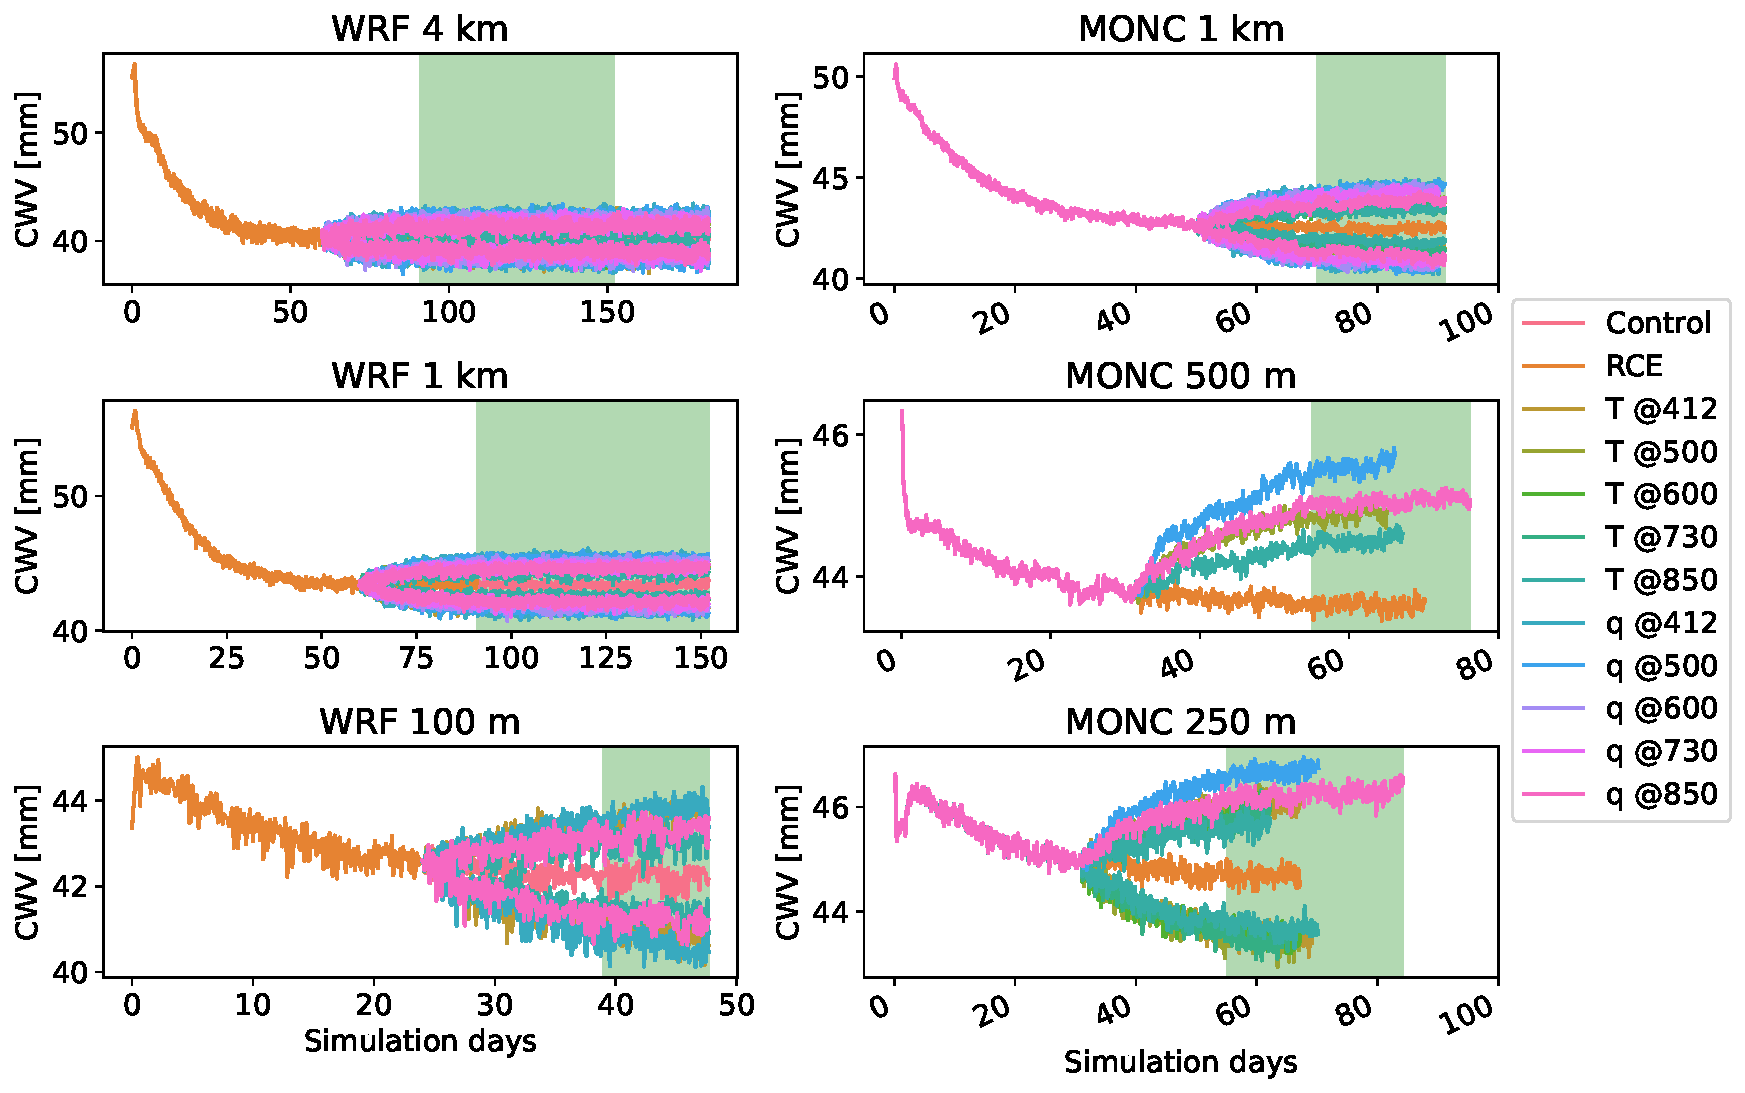
\includegraphics[width=\textwidth]{figures/runs_timeseries.pdf}
    \caption{Time series of water content (spatial mean column water vapor, CWV)
    by grid spacing in WRF and MONC. RCE runs were performed until the columnar
    water content stabilized. At this point the perturbations were introduced,
    and the model was run until all perturbed runs had also reached equilibrium.
    The parts of the time axes highlighted in green show the ``RCE region'' over
    which mean profiles were calculated for comparison. For the MONC runs, the
    highlighted region shows the maximum range of RCE regions, since RCE regions
    were defined as the last 20 days in each simulation for 1 km runs and the
    last 10 days in each simulation for the 500 m and 250 m runs. To reduce the
    number of colors required, positive and negative perturbations use the same
    color.}
    \label{fig:rce_pw}
\end{figure}

Mean profiles from the control run in RCE are shown in Figure
\ref{fig:rce_profiles}. The mean states are similar for the two models,
especially considered within the context of larger inter-model comparisons of
RCE states \cite<e.g.>{Hwong_JAMES_2021}. To some extent the similarities may be
due to the idealized treatment of radiation and evaporation used here, but it is
notable that simply by resolving convection explicitly the mean states were
brought into closer agreement than in \citeA{Hwong_JAMES_2021}, in which single
column models used idealised radiation and evaporation, as here, but convection
was parameterized. In Figure \ref{fig:rce_profiles}, moisture content generally
increases with finer resolution for all heights.  MONC is marginally moister and
warmer than WRF. The moisture changes with resolution are modest in terms of
mixing ratios when expressed as relative humidity in the lower part of the free
troposphere above about 900 hPa. We hypothesize that is the result of some
transport from shallow convection. In the WRF runs, at 100 m grid spacing the
profile of relative humidity is fairly uniform with height between $\sim$950 and
$\sim$600 hPa, whereas at 1 km and 4 km grid spacing this part of the atmosphere
is drier, with the 4 km WRF simulation drying to $\sim$60\% relative humidity at
about 800 hPa. The MONC runs also show decreased relative humidity with coarser
resolution, and are drier than the WRF runs in a region around $\sim$600 hPa.
Mean wind profiles for the 100 m run, which had finer vertical resolution, and
was temporally shorter than the other runs, are not as smooth as those for the 1
km and 4 km runs.

\begin{figure}[pth]
    \noindent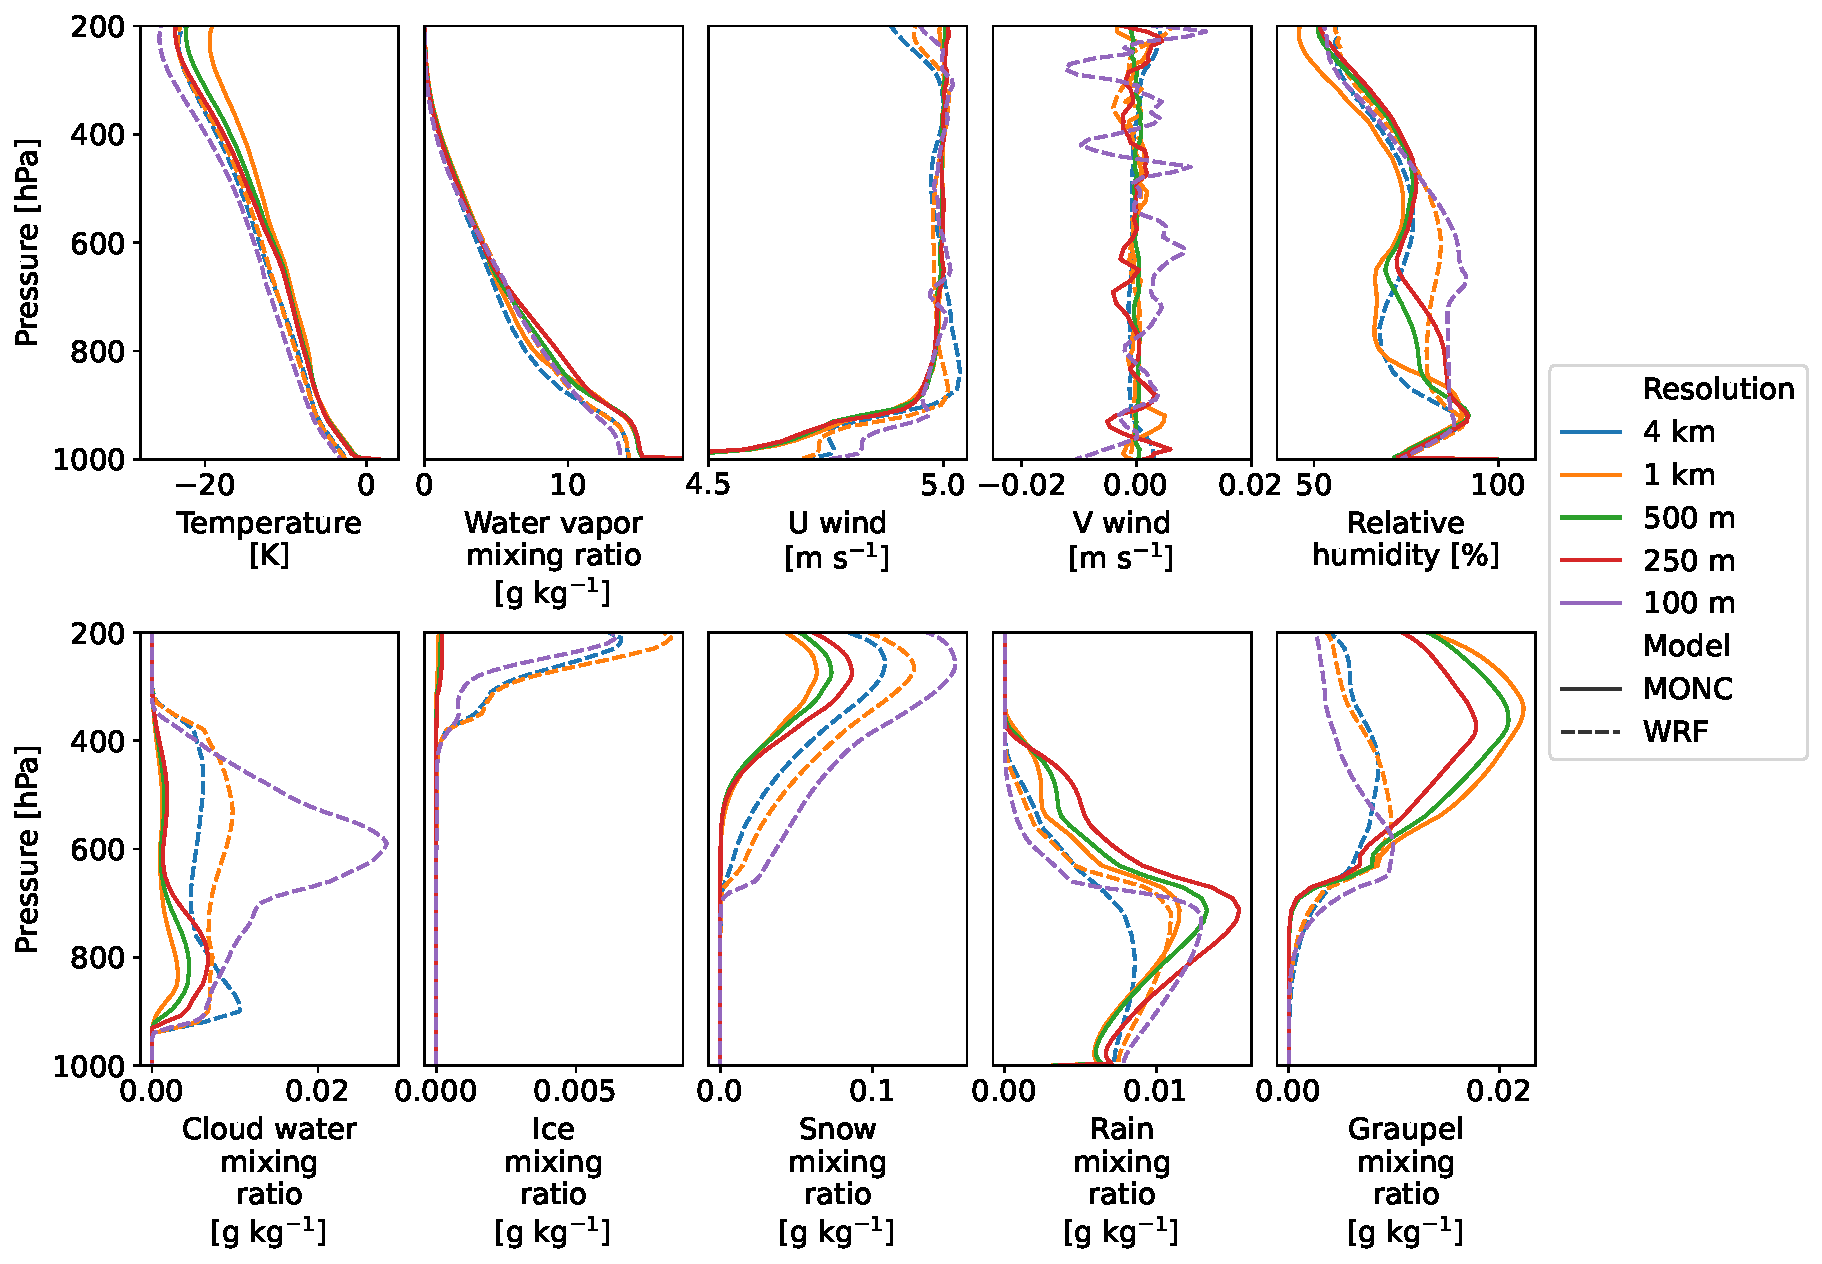
\includegraphics[width=\textwidth]{figures/rce_profiles}
    \caption{Mean profiles for selected variables in the control runs' RCE
    periods, by grid spacing. The water vapor mixing ratio x-axis is truncated
    at 18 g kg$^{-1}$. All plots stop at 200 hPa, meaning that a thin cirrus
    layer that formed at the tropopause in the MONC simulations is not shown
    here. Temperatures are shown as anomalies from a reference moist
    pseudo-adiabat calculated using a surface temperature of 300 K. Mean wind
    profiles for MONC are not shown \todo{THR: can we add these please?}.}
    \label{fig:rce_profiles}
\end{figure}

Hydrometeor profiles were sensitive to resolution (Figure
\ref{fig:rce_profiles}). For the WRF runs, finer resolution resulted in more
rain water mass below $\sim$650 hPa and less above, more cloud droplet and snow
mass, more graupel mass below $\sim$500 hPa and less above, and mixed changes in
ice mass. MONC runs were marginally less sensitive, but the character
of the changes is broadly the same as in WRF, except that MONC at finer
resolution produced more rain at all levels and lower tropospheric graupel was
not particularly affected by resolution. Profile shapes are broadly similar
between WRF and MONC, with perhaps the strongest difference in cloud water, for
which MONC produced significantly less between $\sim$650 and $\sim$450 hPa.
There is a significant difference in the cloud water content between the 4 km
and 1 km grid spacings in WRF, and a particularly marked difference in WRF
between the 1 km and 100 m grids around $\sim$600 hPa. Graupel and snow were
produced at lower heights in WRF than in MONC. In both models, finer resolution
brought more snow at cloud top and less graupel, with relative differences
varying by height. It is unclear whether these microphysical changes are simply
a consequence of mean moisture changes or whether they reflect the impact of
cloud turbulence differences.

\subsection{Convective Organization}

We tested for convective organization, to check whether any of the between-model
or between-resolution differences may be due to some setups developing
organization. To do so, we examined the spatial variance of precipitable water
scaled by its spatial mean (not shown) for both models, and for MONC we also
examined the ``subsidence fraction'', the fractional area of the domain where
the vertically integrated mass-weighted vertical wind is negative (not shown).
These metrics showed no evidence of meaningful organization, which is expected
because we used fixed radiation everywhere without contrasting radiative cooling
profiles in moist and dry regions \cite{Muller_GRL_2015}.

\subsection{Responses to Heating (Temperature) Perturbations}

The responses of the models to perturbations in temperature forcing at 415 hPa
and 850 hPa are shown in Figures \ref{fig:tpert_412} and \ref{fig:tpert_850},
respectively, with results for perturbations at other levels (500, 600, and 730
hPa) shown in the Supplement (Figures \ref{fig:tpert_500}, \ref{fig:tpert_600},
and \ref{fig:tpert_730}). All responses to these perturbations are much smaller
than the differences in the mean profiles owing to resolution (Figure
\ref{fig:rce_profiles}). WRF and MONC produced responses of similar amplitude.
In the temperature, water vapor mixing ratio, and relative humidity fields, MONC
was more likely to show nonlinearity, or differences in responses to positive
and negative perturbations, than WRF at 1 km or 4 km resolutions, with the most
pronounced example being the temperature response in the upper troposphere to a
temperature perturbation at 850 hPa. The 100 m WRF results also show some
nonlinearity in their responses. In the hydrometeor fields, the strongest
nonlinearity is found in the WRF results at 100 m grid spacing. However, there
was a large range of responses at 100 m grid spacing (Figures
\ref{fig:var_T_412} and \ref{fig:var_T_850}), meaning that the discrepancies
between responses for positive and negative perturbations are not necessarily
caused by nonlinearity but rather by noise in the response signal for these
hydrometeor mixing ratios.

\begin{figure}[pth]
    \noindent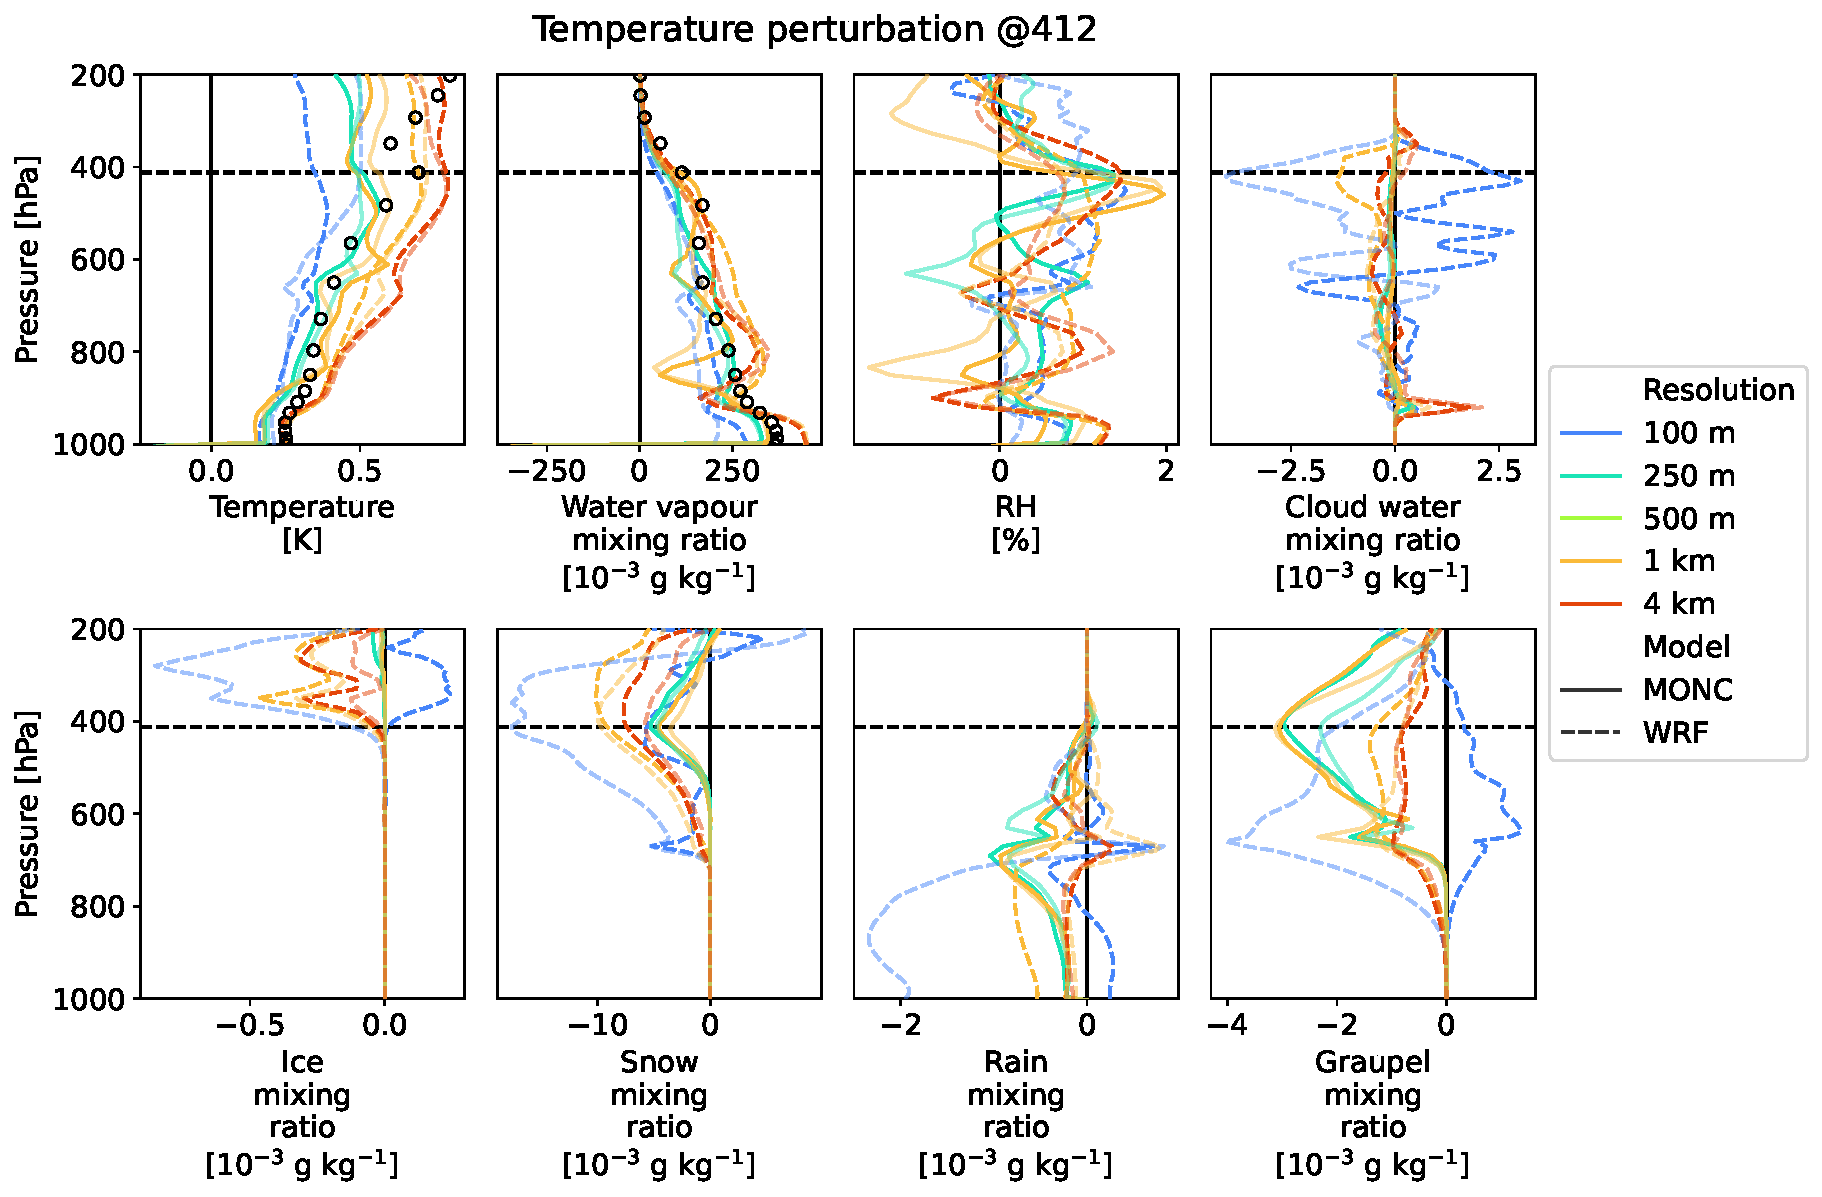
\includegraphics[width=\textwidth]{figures/pert_diffs_T_0.5_@412}
    \caption{Differences in model values by pressure, after a perturbation
    forcing of amplitude 0.5 K was introduced in the potential temperature
    tendency field at 412 hPa (415 hPa for MONC). The solid vertical black line
    shows zero difference. The dashed horizontal line shows the approximate
    level of maximum perturbation. Responses to positive perturbations are shown
    with opaque lines, while responses to negative perturbations are shown with
    semi-transparent lines. Responses to negative perturbations have been
    multiplied by $-1$, so they overlay responses to positive perturbations if
    the positive and negative responses are symmetrical. Black circles show the
    responses to the same perturbation recorded by \citeA{Kuang_JAS_2010}.}
    \label{fig:tpert_412}
\end{figure}

\begin{figure}[pth]
    \noindent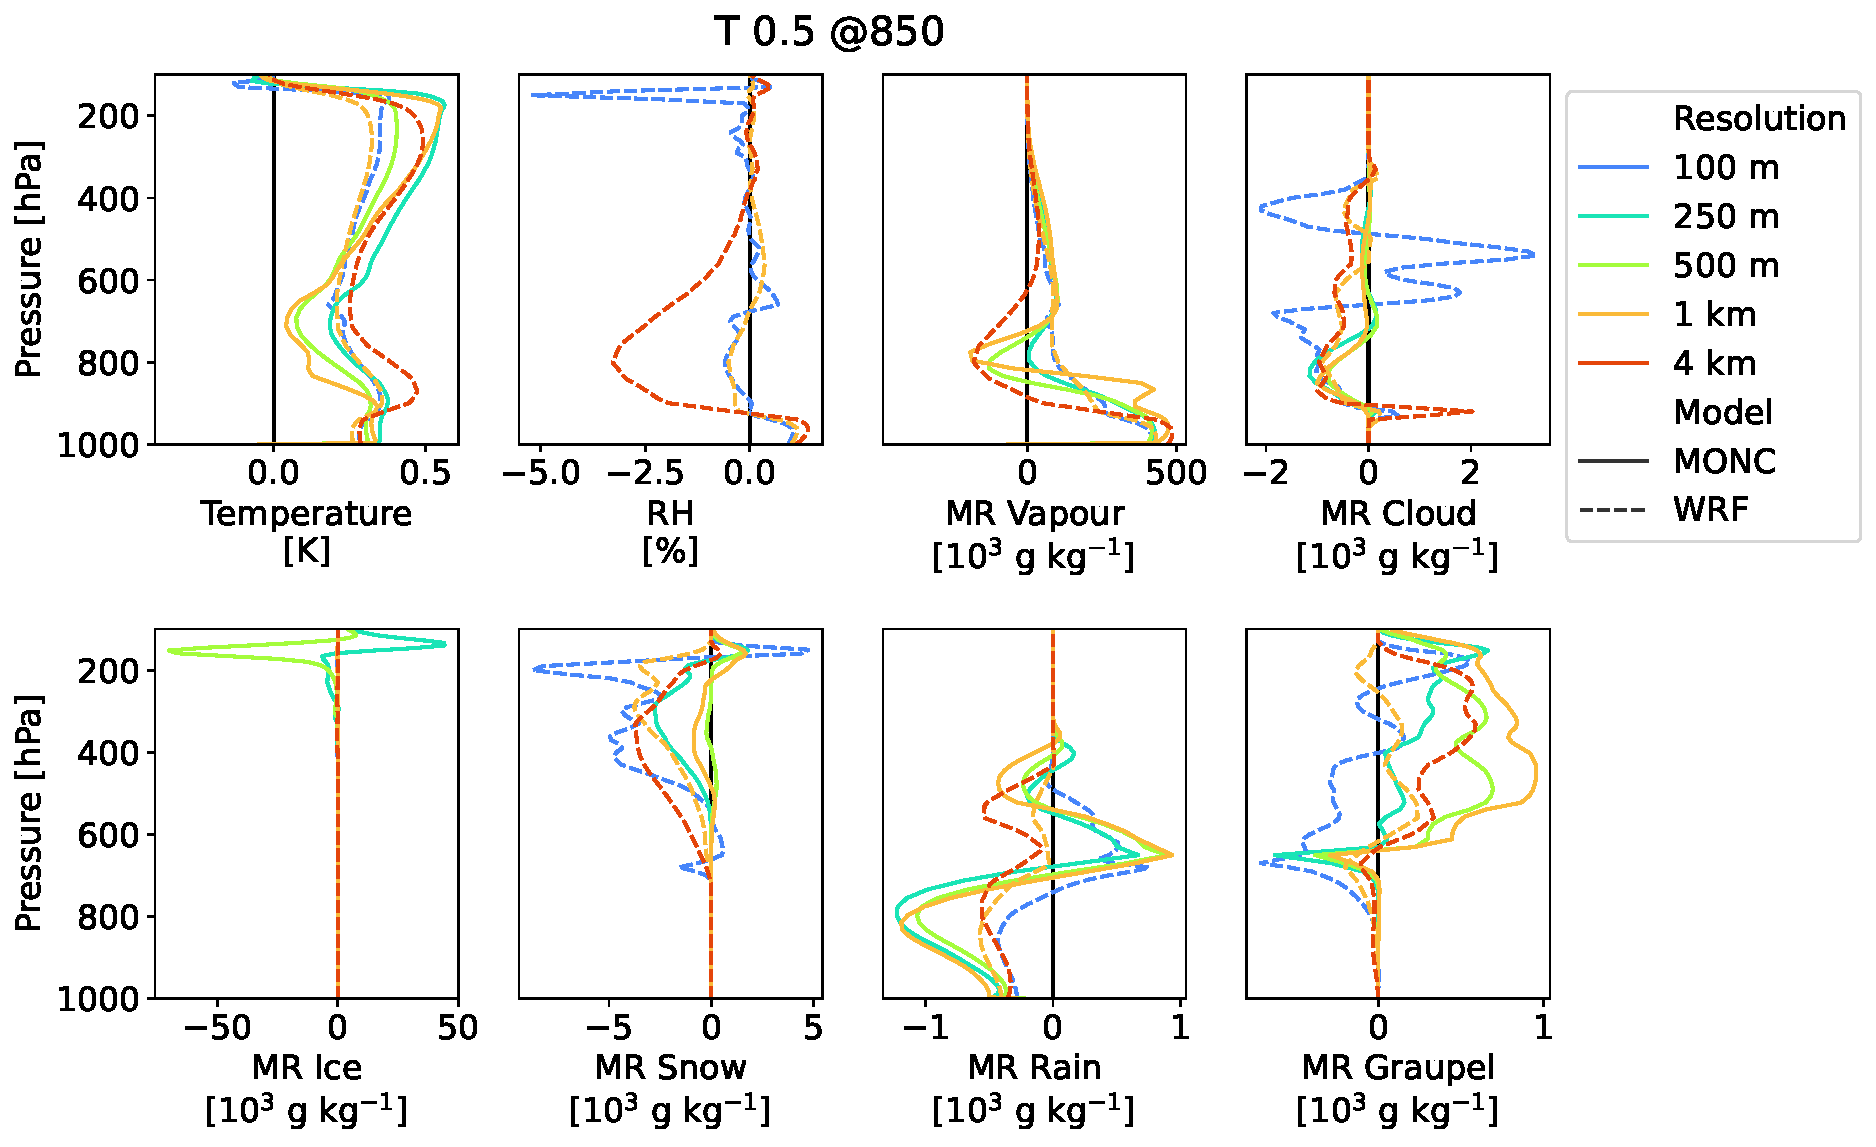
\includegraphics[width=\textwidth]{figures/pert_diffs_T_0.5_@850}
    \caption{As in Figure \ref{fig:tpert_412}, but for a temperature
    perturbation at 850 hPa.}
    \label{fig:tpert_850}
\end{figure}

\subsubsection{Temperature Responses}

In response to temperature perturbations, the temperature response tends to
increase with height from the surface to a maximum just below the perturbation
level, then decreases around the perturbation level before once more increasing
with height. This structure is most apparent in the responses to perturbations
in the middle levels (500, 600, 730 hPa), and it is not apparent in the
responses for a perturbation at the low level of 850 hPa. This ``dog leg''
structure is also often more marked in MONC than in WRF which gives a smoother
temperature response in the vertical. The sub-km resolution runs with MONC also
produce smoother responses than the 1 km runs.

\subsubsection{Moisture Responses}

The moisture responses to the temperature perturbations again appear smoother
vertically from WRF than from MONC \todo{SS: Is that all?  Can we add to this
sentence to make it a statement of the key outcomes?}. The temperature
perturbations at 415 and 850 hPa produce the strongest differences among
the various runs. In some cases (WRF at 4 km grid spacing and MONC at 1 km and
500 m), the 850-hPa perturbation can induce a drying response at and just above
the perturbation level. With WRF, this response becomes a moistening at finer
resolution. With MONC, the drying is a little less marked at 500 m than at 1 km
grids, and at 250 m the response was zero at this level. For the temperature
perturbation at 850 hPa, moistening in the boundary layer reduces for finer
resolutions in WRF, and to a lesser extent for MONC. 

A temperature perturbation at 415 hPa produces a minimum in the moistening in
the WRF runs at around 900 hPa. In MONC there is a similarly pronounced minimum,
a little higher at about 850 hPa, seen in the 1 km run. Similar comments apply
for 500 and 600 hPa perturbations as for 412 hPa. There is often a small minimum
in the moistening responses around or at the perturbation level itself,
particularly for perturbations applied at lower levels (at higher levels a
second minimum tends to appear below the perturbation). For a temperature
perturbation at 730 hPa, the moistening minimum around the perturbation level is
pronounced in MONC and reaches around zero, but it does not produce the drying
seen when the perturbation is applied at 850 hPa. One way to think about the
drying with perturbations at 850 hPa is that the minimum we see consistently
just above the boundary layer combines with the minimum that we often see at or
below the perturbation level.

\subsubsection{Hydrometeor Responses}

The two models show responses in hydrometeor content that are broadly similar in
character, although there are sometimes large differences in response
magnitudes, and the models do not agree on how responses change with resolution.
For the temperature perturbation at 850 hPa in WRF, there is generally a
reduction of rain below the freezing level; MONC shows a stronger reduction than
WRF below the freezing level but an increase around the freezing level, which is
a feature not seen in the WRF results. Except for a near-surface increase, a
reduction in cloud liquid water also occurs, and this is over a deeper layer in
WRF than in MONC. There is also some reduction to snow and increase in graupel
at upper levels. 

For WRF runs with temperature perturbations at lower \todo{RSP: I think this
should be upper?} levels, the profiles of liquid water changes have reductions
with minima that are aligned with or just above the perturbation height. As the
perturbation level increases in the WRF runs, a maximum in liquid water changes
appears between the perturbation level and the surface. The 4 km WRF runs in
particular show a sharp increase in cloud water at about 900 hPa under all
temperature perturbations. The responses of hydrometeors in MONC have a broadly
similar character, but some of the amplitudes are quite different. There are
similar amplitudes to WRF for rain, but weaker responses in liquid water, ice
and snow. MONC responded more strongly for graupel, however, especially in
response to perturbations at 415 and 500 hPa. A positive temperature
perturbation generally reduces graupel content except for some increases at high
levels when the perturbation was closer to the surface. There are some changes
in responses with grid length. For the WRF runs the rain changes tend to
increase in magnitude with finer resolution, while the MONC responses are more
similar. For MONC the liquid water reductions are stronger at 250 m than at 1 km
spacings, and for temperature perturbations at lower levels snow is also more
strongly reduced at 250 m than at 1 km grid spacing. The changes in graupel
become weaker with finer resolution in MONC runs yet stronger with decreasing
grid spacing for WRF runs. 

\todo{RSP: to follow on from Steve's comment at the
start of the section it may be good to have a short summary at the end too. The
main points seem to be: broadly similar character of responses in the 2 models
but sometimes with quiet different amplitudes and presumably attributable to
difference in the microphysics representation. And: the lack of agreement
between the models about how responses change with resolution.}

\subsection{Responses to Moistening (Humidity) Perturbations}

The responses of the models to perturbations in moisture at 415 and 850 hPa
are shown in Figures \ref{fig:qpert_412} and \ref{fig:qpert_850}, respectively,
while perturbations for 500 hPa, 600 hPa, and 730 hPa, are shown in Figures
\ref{fig:qpert_500}, \ref{fig:qpert_600}, and \ref{fig:qpert_730}, respectively.
Several elements of these results are similar to the results for temperature
perturbations: moisture and hydrometeor responses to moisture perturbations are
again smaller than the differences in the mean profiles due to resolution
\todo{Steve: Bob is correct these can be compared because neither involve units
of time}. WRF and MONC produced responses of similar amplitude, except for cloud
liquid water and ice where the changes in MONC were much smaller; and MONC shows
more nonlinearity in temperature, water vapor and relative humidity responses
than WRF does at 1 km and 4 km grid spacings. MONC relative humidity seems to be
particularly prone to non-linear responses. Similar to the responses to the
temperature perturbations, the strongest apparent nonlinearity after moisture
perturbations is in the hydrometeor fields and especially for the 100 m grid
spacing WRF responses, but as for the temperature perturbations there was a
large range in responses (Figures \ref{fig:var_q_412} and \ref{fig:var_q_850}).

\begin{figure}[pth]
    \noindent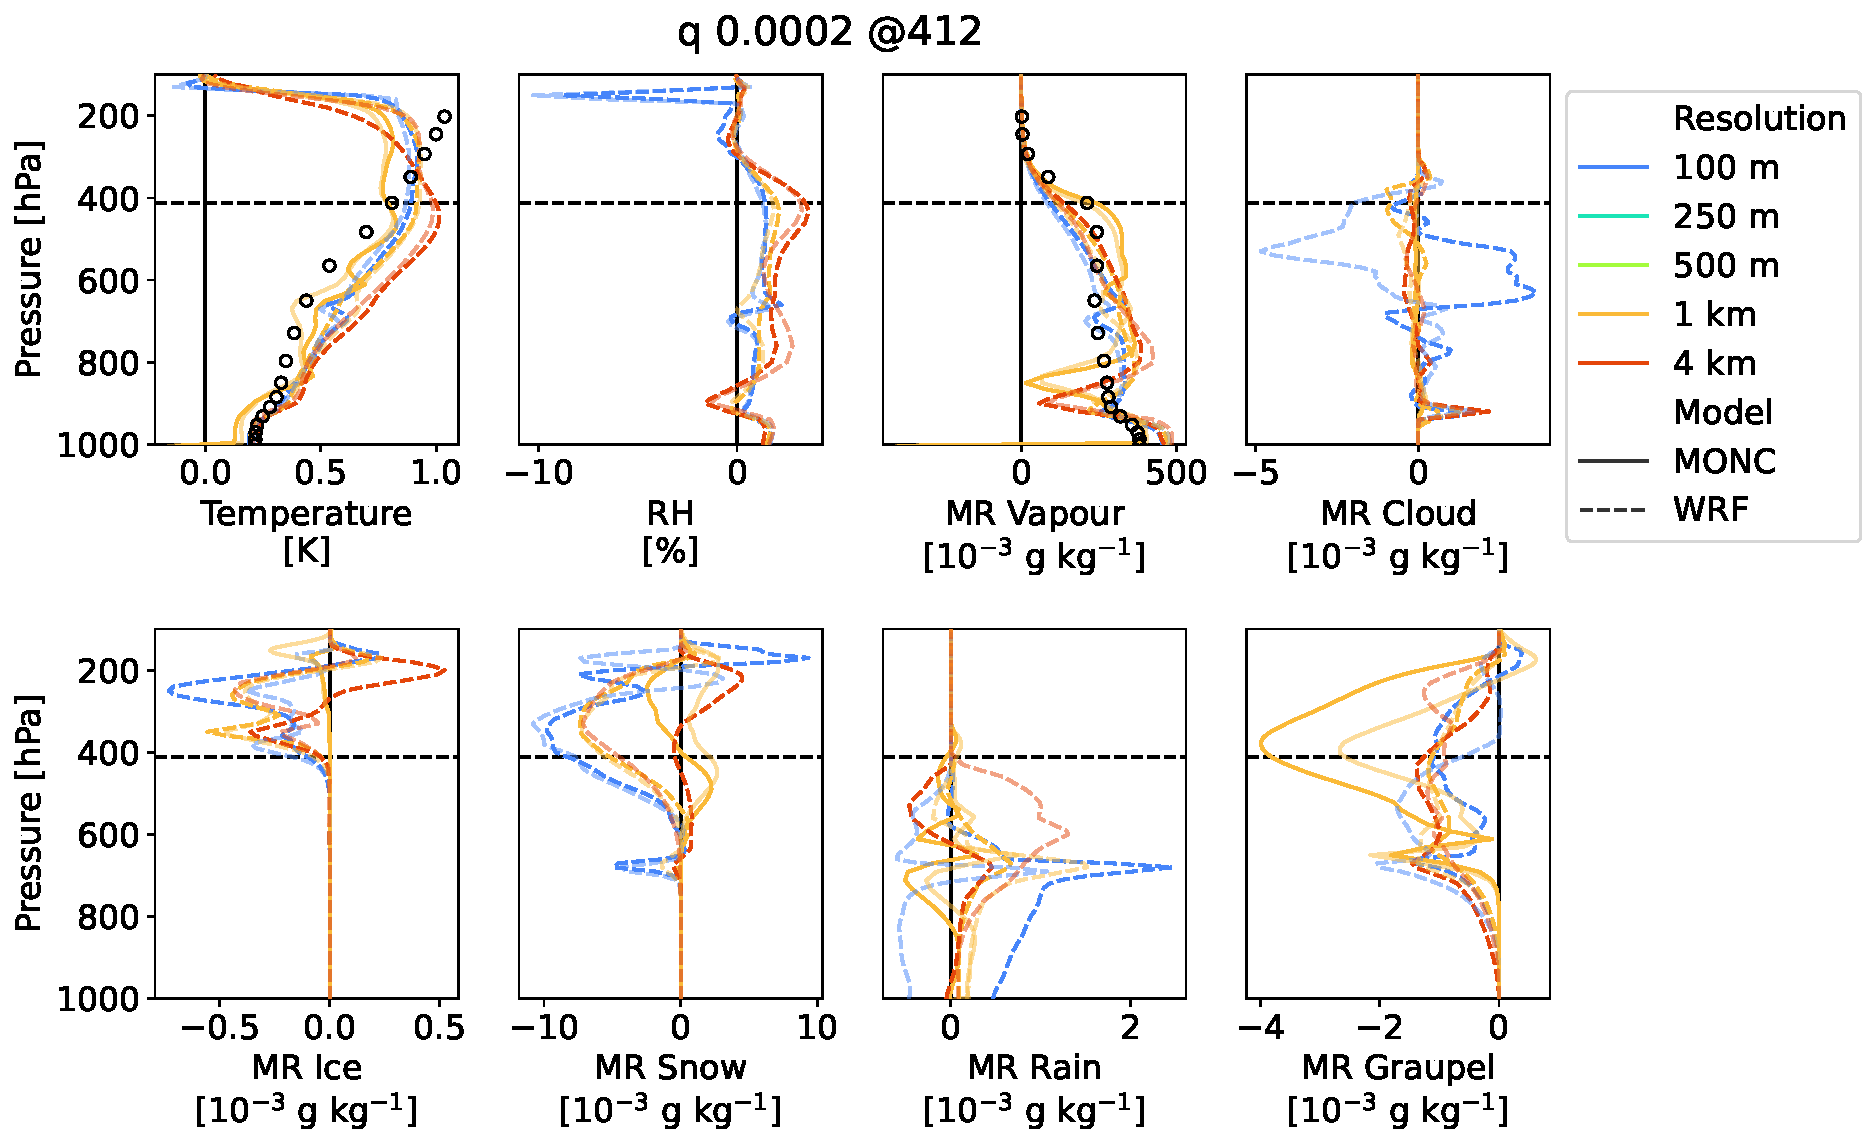
\includegraphics[width=\textwidth]{figures/pert_diffs_q_0.0002_@412}
    \caption{As for Figure \ref{fig:tpert_412}, but for differences in model
    values by pressure, after a perturbation forcing of amplitude 0.2 g
    kg$^{-1}$ was introduced in the water vapor mixing ratio tendency field at
    412 hPa (415 hPa for MONC).}
    \label{fig:qpert_412}
\end{figure}

\begin{figure}[pth]
    \noindent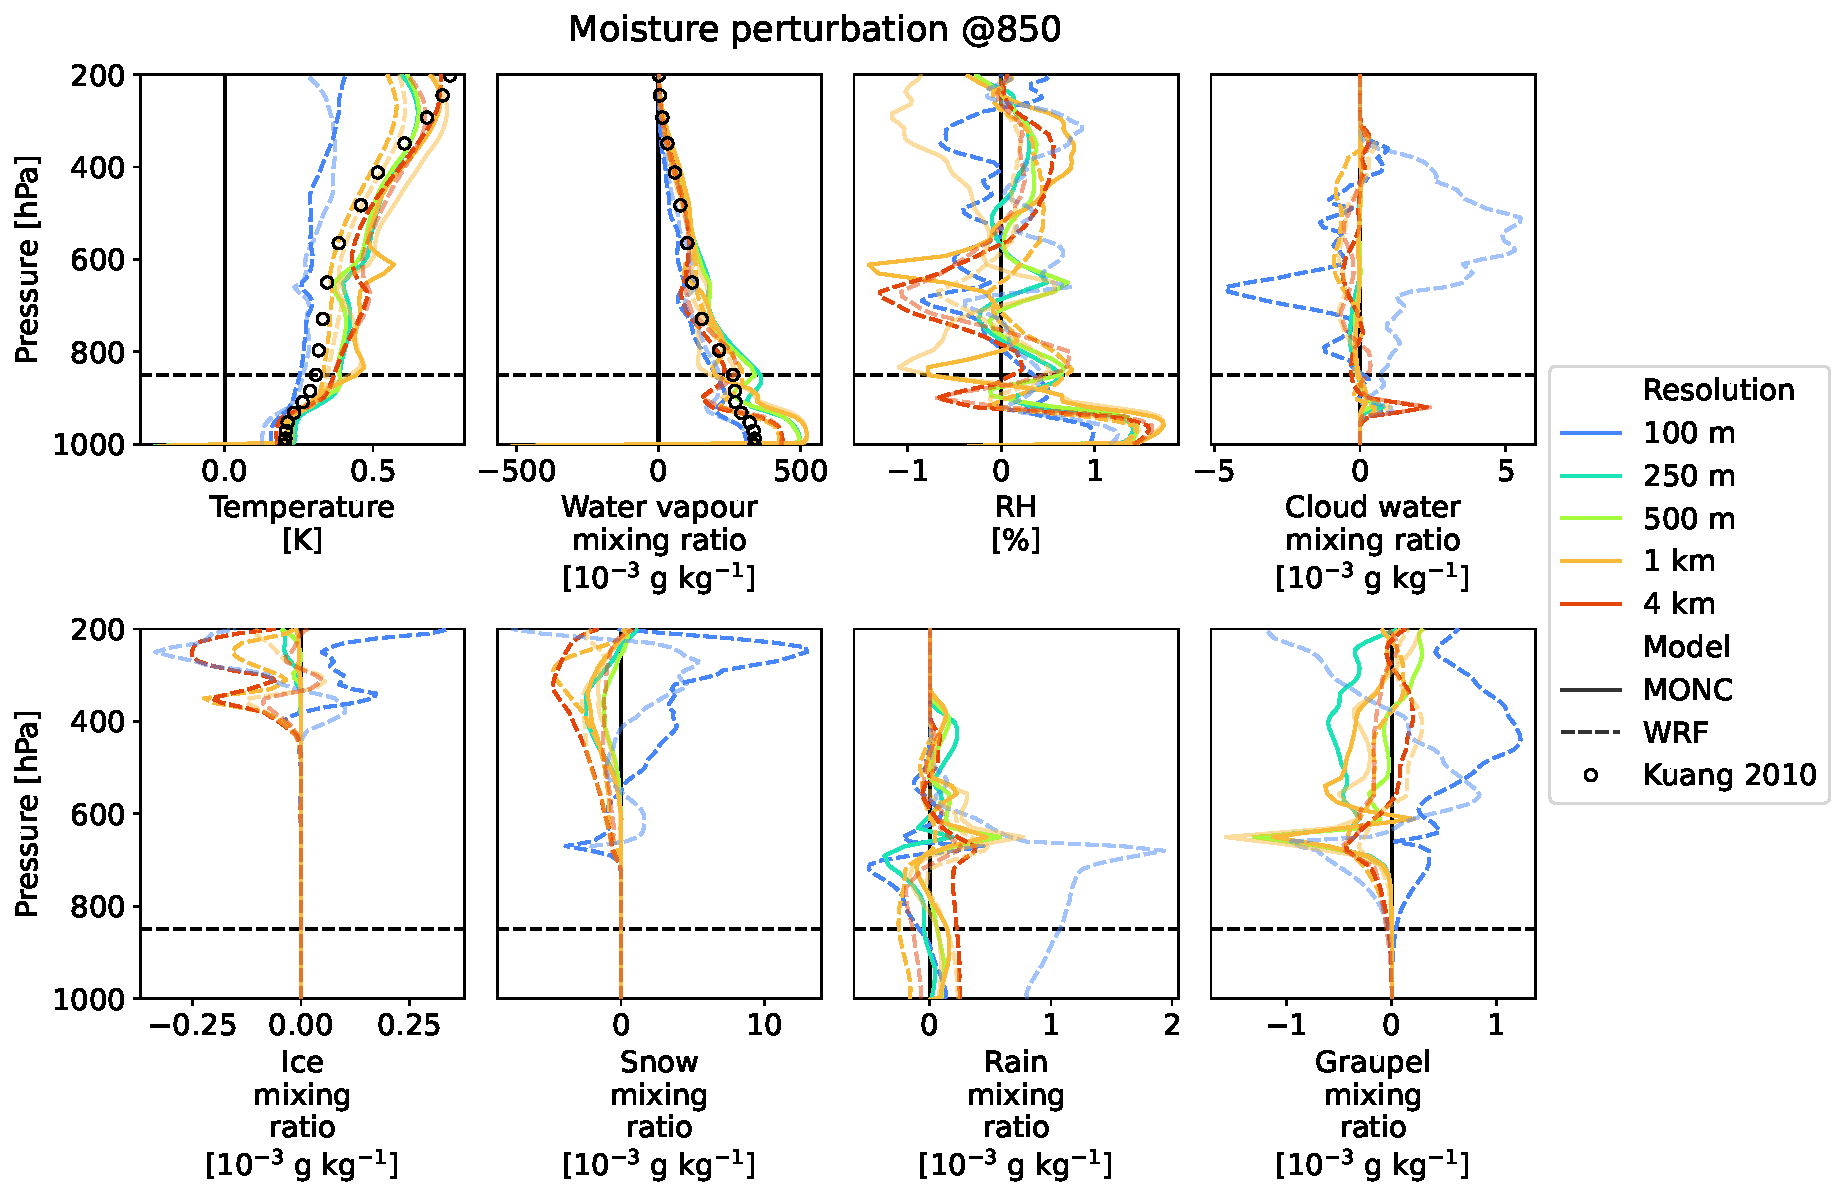
\includegraphics[width=\textwidth]{figures/pert_diffs_q_0.0002_@850}
    \caption{As in Figure \ref{fig:qpert_412}, but for a water vapor mixing
    ratio perturbation at 850 hPa.}
    \label{fig:qpert_850}
\end{figure}

\subsubsection{Temperature Responses}

With moisture perturbations, temperature increases in the boundary layer are
very consistent between resolutions in WRF, but the free tropospheric
temperature increases are stronger at coarser resolution and less strong for
100-m grid spacing across the whole profile. Particularly notable is the
increase in the temperature increase between 1 km and 4 km grid spacings for a
perturbation at 412 hPa. MONC responses show a similar response below about 600
hPa and above about 850 hPa, but outside this region the responses for higher
resolution runs are stronger than those for 1-km runs. The boundary-layer
temperature increases are very consistent between WRF and MONC. The
free-tropospheric increases are stronger in MONC for a low-level moisture
perturbation and weaker for an upper-level moisture perturbation.

\subsubsection{Moisture Responses}

The WRF responses of specific humidity to moisture perturbations have minima at
around 900 hPa and to a lesser extent around 650 hPa \todo{SS: regardless of the
forcing level?  State this}. These minima are modest at fine grid spacing, but
at coarse resolution the lower minimum becomes stronger even for perturbations
made at upper levels. It does however remain positive for positive
perturbations. Such minima are also present in MONC, the lower level one being a
little higher and much more pronounced than in WRF at the same grid spacings,
and the MONC responses also remaining positive for positive perturbations.

\subsubsection{Hydrometeor Responses}

There are nonlinearities in the hydrometeor responses, with the most obvious
case that of rain mixing ratios. With some exceptions, increased moisture
tendency shows a small reduction in cloud liquid water across the whole profile
but an increase close to the surface, reductions in ice in the high troposphere,
and reductions in snow above the perturbation level. Graupel is consistently
strongly reduced around 600 hPa, but there are responses with opposite signs in
the upper levels. The responses of hydrometeors in MONC are generally weaker
than WRF for liquid water, ice and snow. MONC responds more strongly for
graupel, however, especially in response to higher level perturbations where
nonlinearities are evident.

\section{Conclusions}
\label{sec:conclusions}

In this work we examined time-averaged responses to temperature and moisture
forcing perturbations in simulated RCE states, using two models at a range of
grid spacings including LES runs without PBL schemes enabled. The aim has been
to test the sensitivity of responses to model parameterizations and resolution.
We now return to the research questions we laid out in the introduction and
examine how our findings have addressed them.

We sought a ``truth'' response or benchmark results against which other models
could be tested. The linear responses in our results are sensitive to model
resolution and model used, but do show a tendency to produce smoother vertical
structures and indications of convergence as grid spacing is reduced. Responses
in temperature and moisture content are more robust than those for hydrometeors,
which are presumably influenced also by the different choices of microphysical
parameterizations. The temperature and water vapor responses also tend to be
closer to the results of \citeA{Kuang_JAS_2010} as grid spacing becomes finer,
especially in the lower troposphere below $\sim$600 hPa, indicating that model
disagreement and sensitivity to parameterization choice is reduced at finer
resolutions \todo{YLH: I think Kuang (2010) uses a resolution of 2km, and we have finer resolutions than his, so I am not entirely sure if saying that his is the "truth" that we are aiming for is a fair comparison. Perhaps skip the part about "closer to results of Kuang"}. In the upper troposphere above $\sim$500 hPa, our
highest-resolution results show a smaller mean response than in
\citeA{Kuang_JAS_2010}. The question is, then, what resolution is required to
consider a response a benchmark result?

We can narrow down the grid spacing required to properly represent
convective-scale feedbacks on large scale flows by examining the sensitivity of
the feedbacks to model settings. From our results, it appears that model-based
differences between responses to perturbations do not start to disappear until
the grid spacing below $\sim$1 km and perhaps lower for responses in the upper
troposphere. While apparent convergence at grid spacings less than $\sim$1 km
appears across our results, we note that variability across perturbations was
present and computational limitations precluded us from performing rigorous
convergence tests. Nonetheless, these convergence results do suggest that for
most models, to simulate convectively-coupled dynamics correctly will likely
require better resolution than is currently used in, for example, DYAMOND
\cite{Stevens_PEPS_2019}. Our results also suggest that, in the lower
troposphere, tangent linear responses are similar across the two LES models
tested here, implying they could make reasonable benchmark estimates of model
responses. In the upper troposphere the results diverge more and therefore the
error bars on responses in this region are larger. Responses for larger grid
spacings than $\sim$1 km diverge significantly from the LES responses.

\todo{Yiling, can you help with a comparison of our results to
\citeA{Hwong_JAMES_2021}? Eg. Bob's points: An important points will be to say
that the differences between responses for different parameterizations are
larger than any uncertainties that we believe are present in defining the
"truth" response. Also, the conclusions here are not the right place to
re-evaluate everything in that paper, but it might be useful to finish this new
paper by commenting on one or two example responses seen there. i.e. in the
earlier paper we could only say that scheme X had such and such a response that
was unusual or a little suspicious but now that we have done the new study we
can now say that we think this type of response from scheme X is actually just
plain wrong. A related question is whether the response is dominated by the
modelled convection itself, or whether it might be sensitive to the
specification of surface properties in an idealized modelling setting.}

\todo{YLH: i have added the following paragraph, please modify as you see fit}

A comparison of our findings with those of the SCM responses in Hwong et al. (2021) reveals several observations. The variations in responses across different convective parameterizations in \citeA{Hwong_JAMES_2021} are generally more pronounced than the uncertainties we estimate within our CRM and LES responses, as well as between the two models. This is particularly noteworthy given the authors’ hesitation to regard Kuang’s (2010) 2-km CRM results as the definitive “truth,” on the grounds that CRM outcomes can be sensitive to model resolution. Hence, the relatively more consistent responses across different resolutions in our study provide confidence in the robustness of our results and offer a clearer perspective on what constitutes a “correct” response. This suggests that high-resolution model outputs can serve as a valuable benchmark for identifying substantial deficiencies in convective parameterizations, particularly when the latter deviate significantly from the responses observed in our simulations. For instance, the pronounced kinks frequently observed in the SCM responses—especially near critical atmospheric levels such as the freezing level and cloud base—appear less prominent or even disappear at finer resolutions in our results, underscoring the problematic threshold-like behavior of convective parameterizations. However, this conclusion does not hold uniformly throughout the entire atmospheric column. As noted earlier, the responses in our high-resolution simulations become increasingly uncertain at higher altitudes, at times exhibiting a spread that exceeds those of the SCMs in \citeA{Hwong_JAMES_2021}. For instance, the temperature response above 300 hPa to a moisture perturbation at 850 hPa appears to show greater variability than the corresponding spread observed in the SCMs. This suggests that in the upper troposphere, the influence of other parameterization schemes—most probably the microphysics scheme—becomes increasingly dominant, surpassing the impact of any convective scheme employed in a model.


In summary, the key conclusions of our study are as follows:

\begin{enumerate}
    \item For most models, correct simulation of convectively-coupled dynamics
    requires a grid spacing of lower than $\sim$1 km.
    \item The linear responses of the two LES models tested here could
    reasonably be used as ground truth for GCM scheme testing.
\end{enumerate}

Some caveats and limitations apply to our study.  Because we used perturbed
forcing on an RCE base, the conclusions apply for deep convection, but finer
resolutions would be required for application to shallow or mid-level
convection.

\section{Open Research}

% AGU requires an Availability Statement for the underlying data needed to
% understand, evaluate, and build upon the reported research at the time of peer
% review and publication.

% Authors should include an Availability Statement for the software that has a
% significant impact on the research. Details and templates are in the
% Availability Statement section of the Data and Software for Authors Guidance:
% \url{https://www.agu.org/Publish-with-AGU/Publish/Author-Resources/Data-and-Software-for-Authors#availability}

% It is important to cite individual datasets in this section and, and they must
% be included in your bibliography. Please use the type field in your bibtex file
% to specify the type of data cited. Options include [Dataset], [Software],
% [ComputationalNotebook], [Collection].
% Example:
%
%@misc{https://doi.org/10.7283/633e-1497,
%  doi = {10.7283/633E-1497},
%  url = {https://www.unavco.org/data/doi/10.7283/633E-1497},
%  author = {de Zeeuw-van Dalfsen, Elske and Sleeman, Reinoud},
%  title = {KNMI Dutch Antilles GPS Network - SAB1-St_Johns_Saba_NA P.S.},
%  publisher = {UNAVCO, Inc.},
%  year = {2019},
%  type = {dataset}
%}

\bibliography{library}

\newpage
\section*{Appendix}
\setcounter{figure}{0}
\renewcommand{\thefigure}{A\arabic{figure}}

\begin{figure}[pth]
    \noindent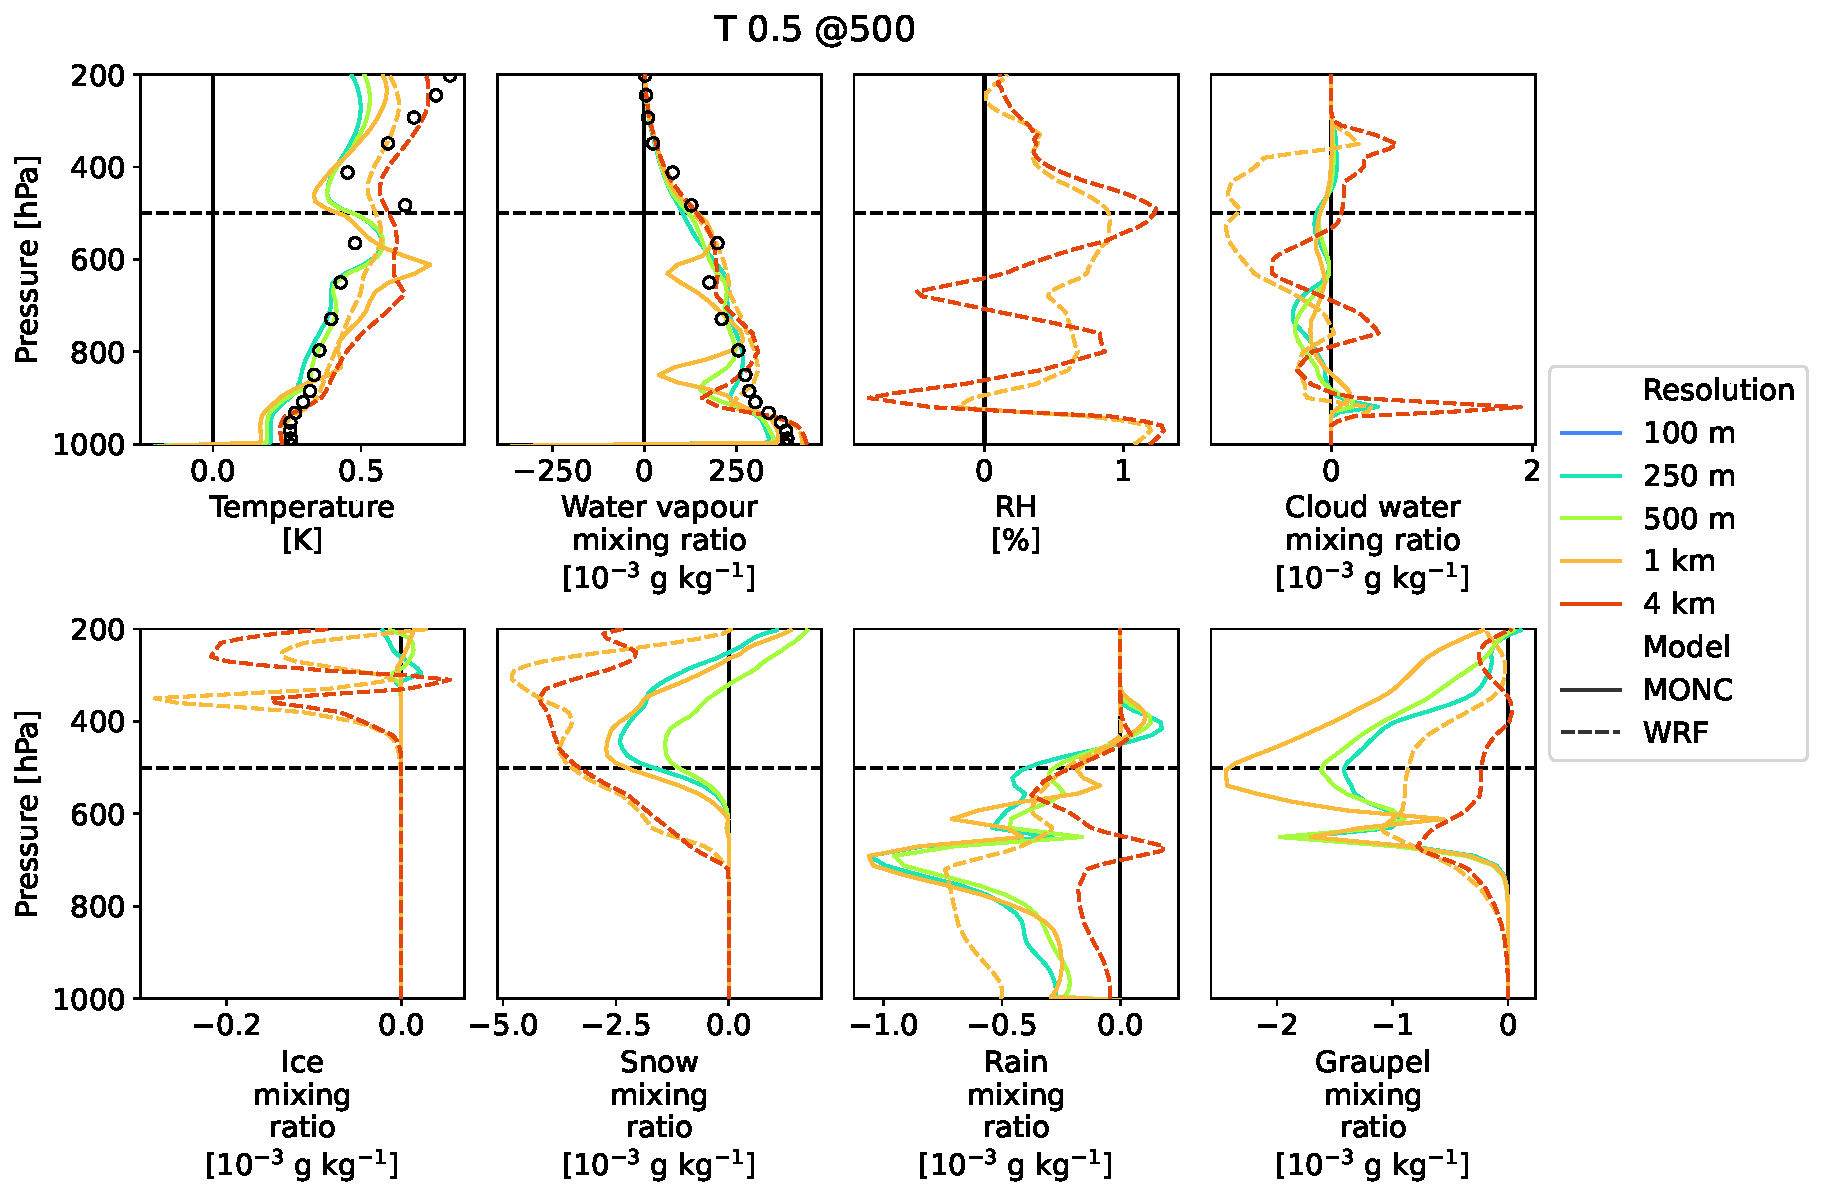
\includegraphics[width=\textwidth]{figures/pert_diffs_T_0.5_@500}
    \caption{As in Figure \ref{fig:tpert_412}, but for a temperature
    perturbation at 500 hPa, and with black circles showing the responses of
    \citeA{Kuang_JAS_2010} to a temperature perturbation at 483 hPa.}
    \label{fig:tpert_500}
\end{figure}

\begin{figure}[pth]
    \noindent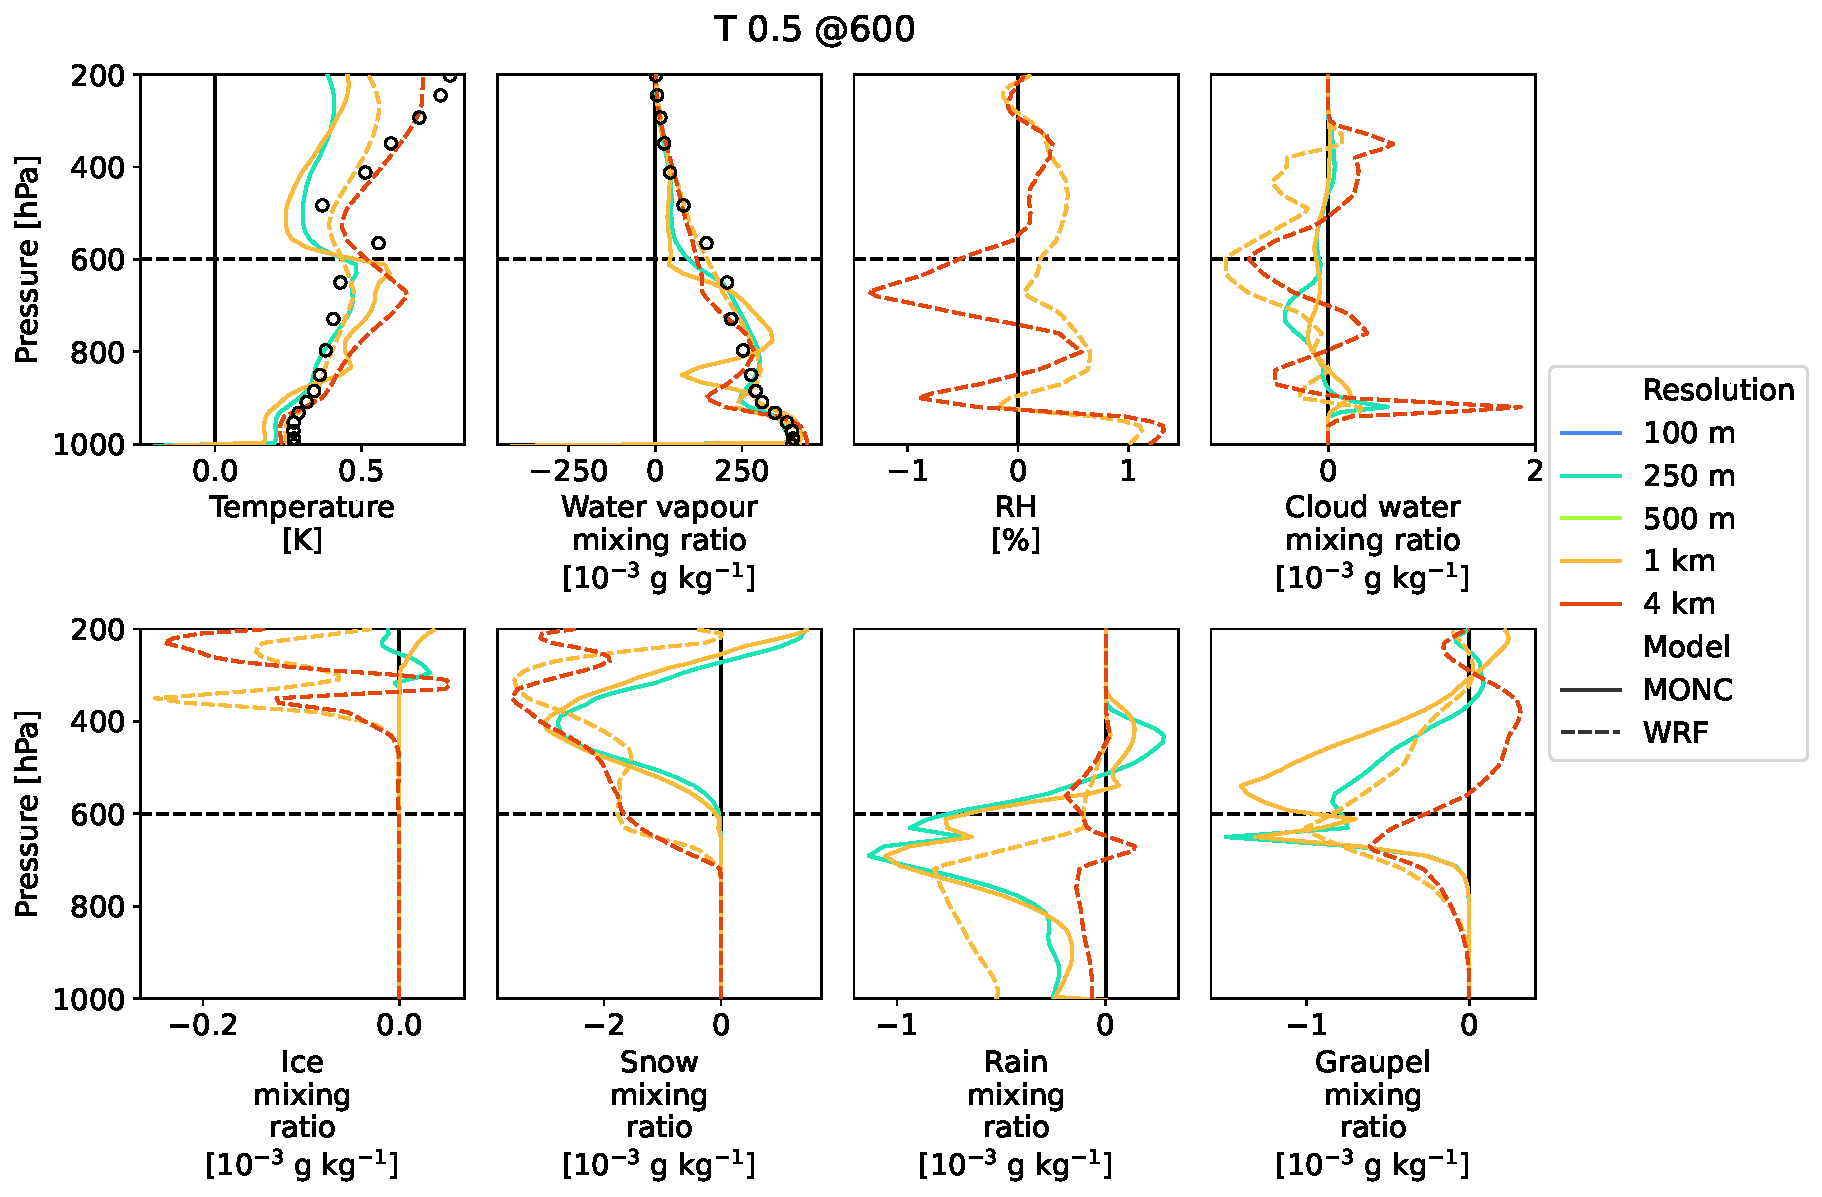
\includegraphics[width=\textwidth]{figures/pert_diffs_T_0.5_@600}
    \caption{As in Figure \ref{fig:tpert_412}, but for a temperature
    perturbation at 600 hPa, and with black circles showing the responses of
    \citeA{Kuang_JAS_2010} to a temperature perturbation at 565 hPa.}
    \label{fig:tpert_600}
\end{figure}

\begin{figure}[pth]
    \noindent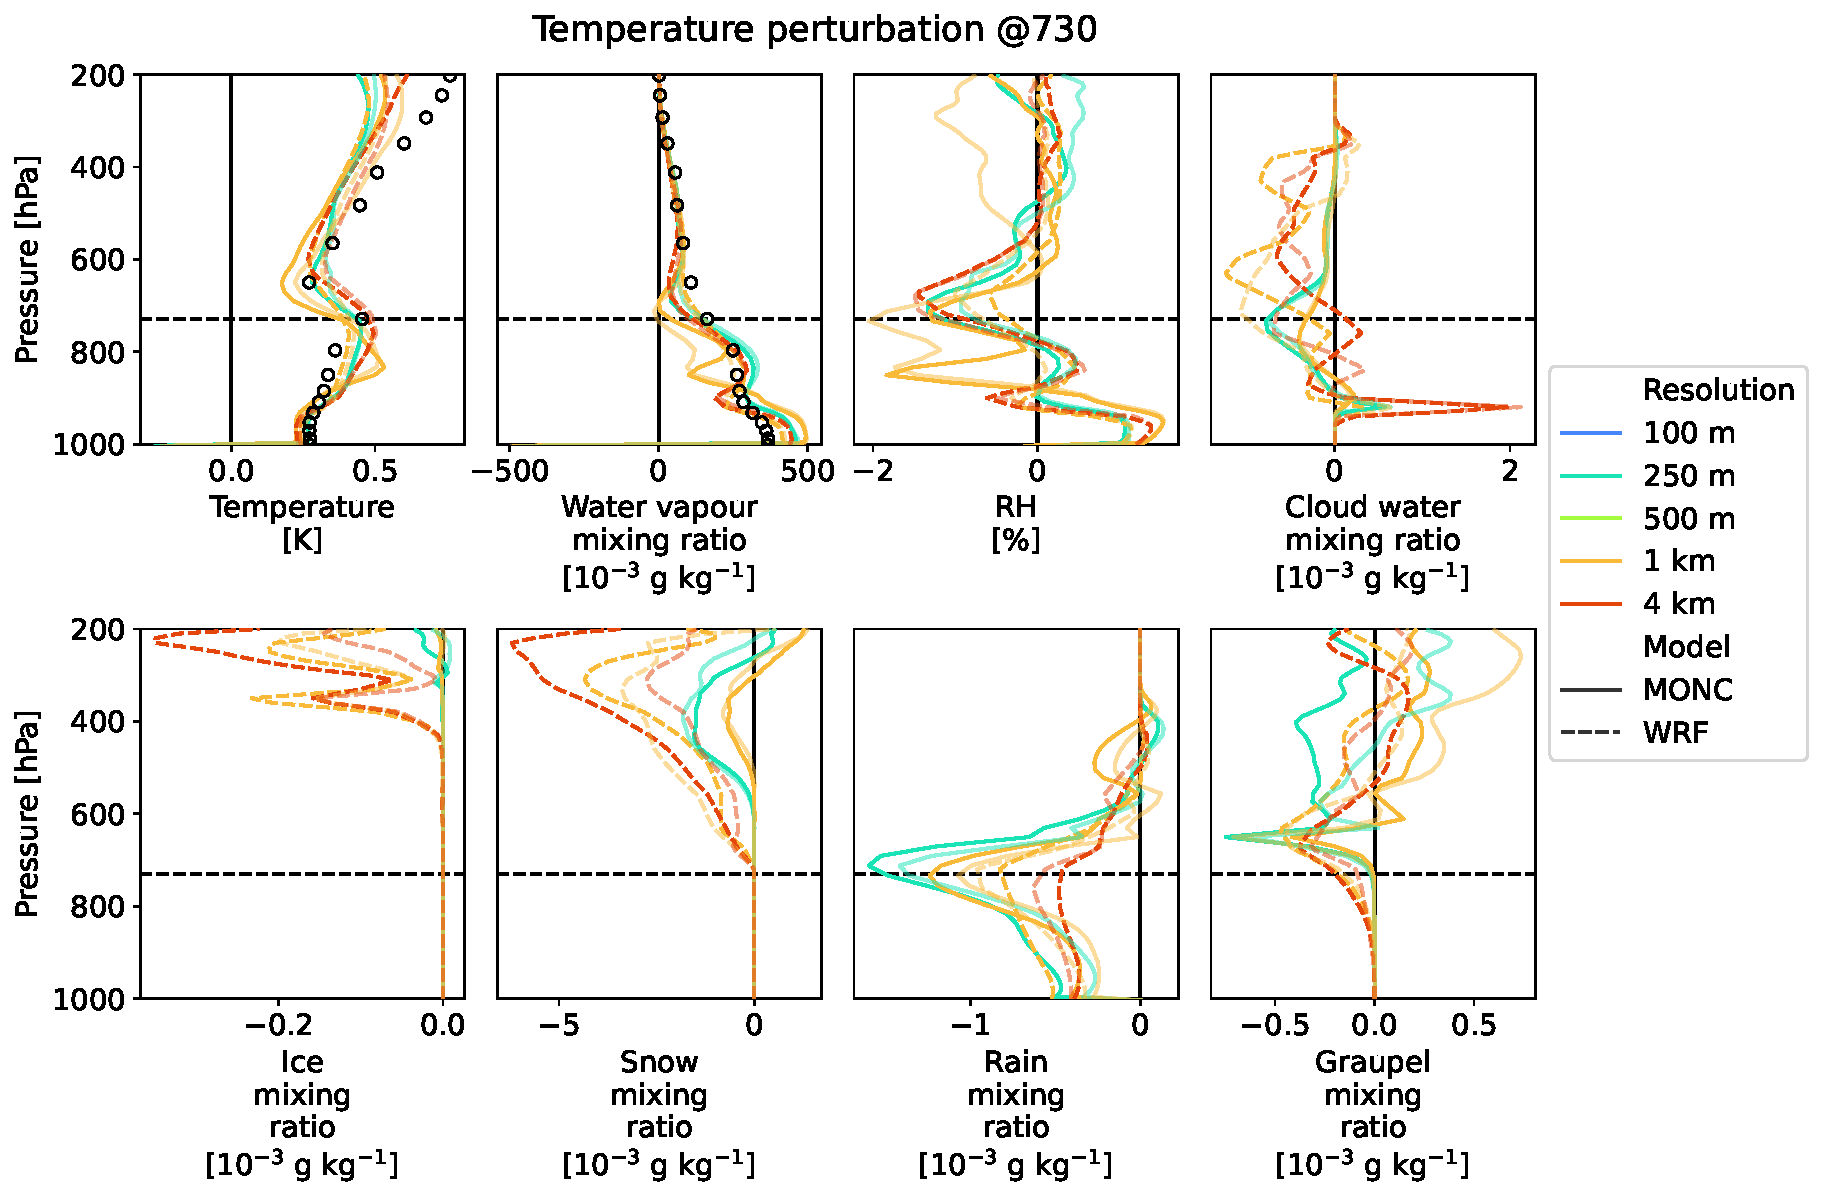
\includegraphics[width=\textwidth]{figures/pert_diffs_T_0.5_@730}
    \caption{As in Figure \ref{fig:tpert_412}, but for a temperature
    perturbation at 730 hPa, and with black circles showing the responses of
    \citeA{Kuang_JAS_2010} to a temperature perturbation at 729 hPa.}
    \label{fig:tpert_730}
\end{figure}

\begin{figure}[pth]
    \noindent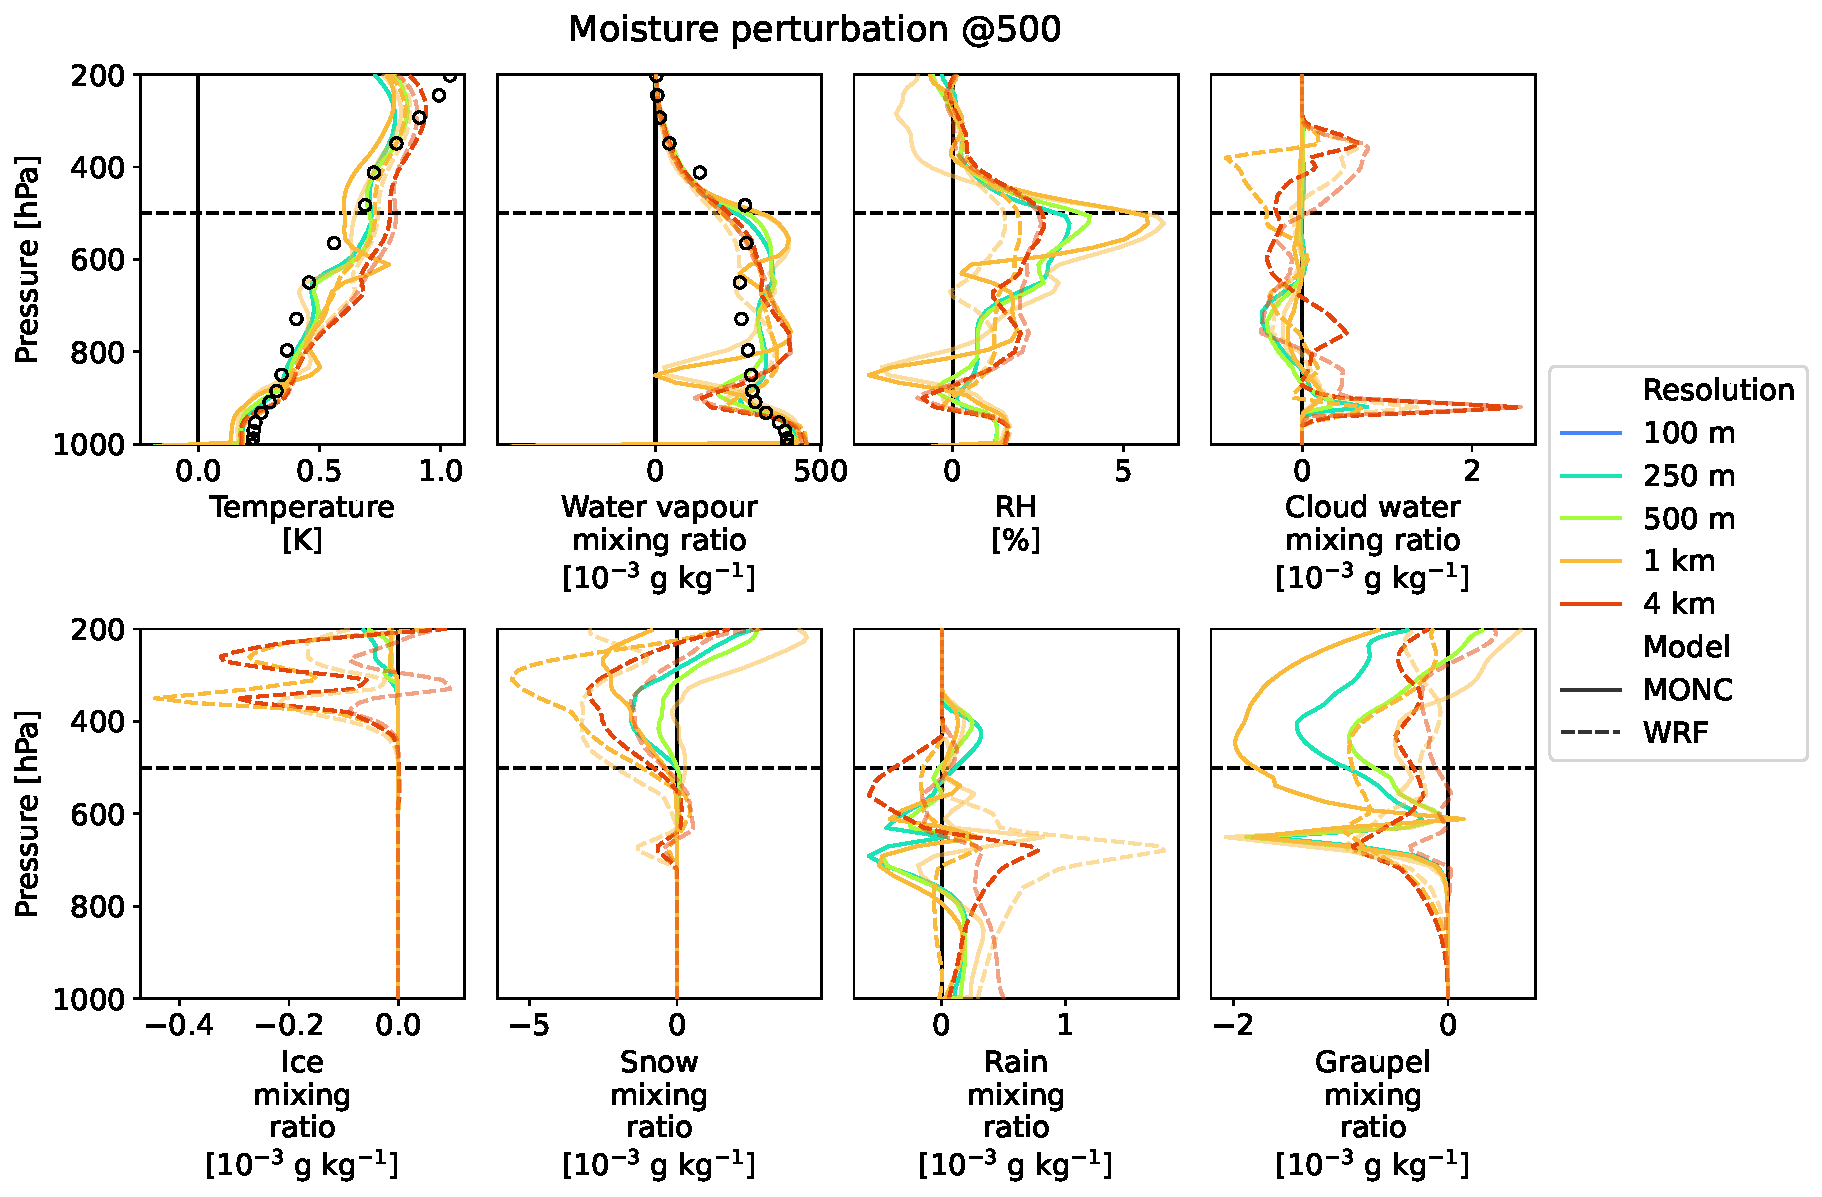
\includegraphics[width=\textwidth]{figures/pert_diffs_q_0.0002_@500}
    \caption{As in Figure \ref{fig:qpert_412}, but for a water vapor mixing
    ratio perturbation at 500 hPa, and with black circles showing the responses
    of \citeA{Kuang_JAS_2010} to a specific humidity perturbation at 483 hPa.}
    \label{fig:qpert_500}
\end{figure}

\begin{figure}[pth]
    \noindent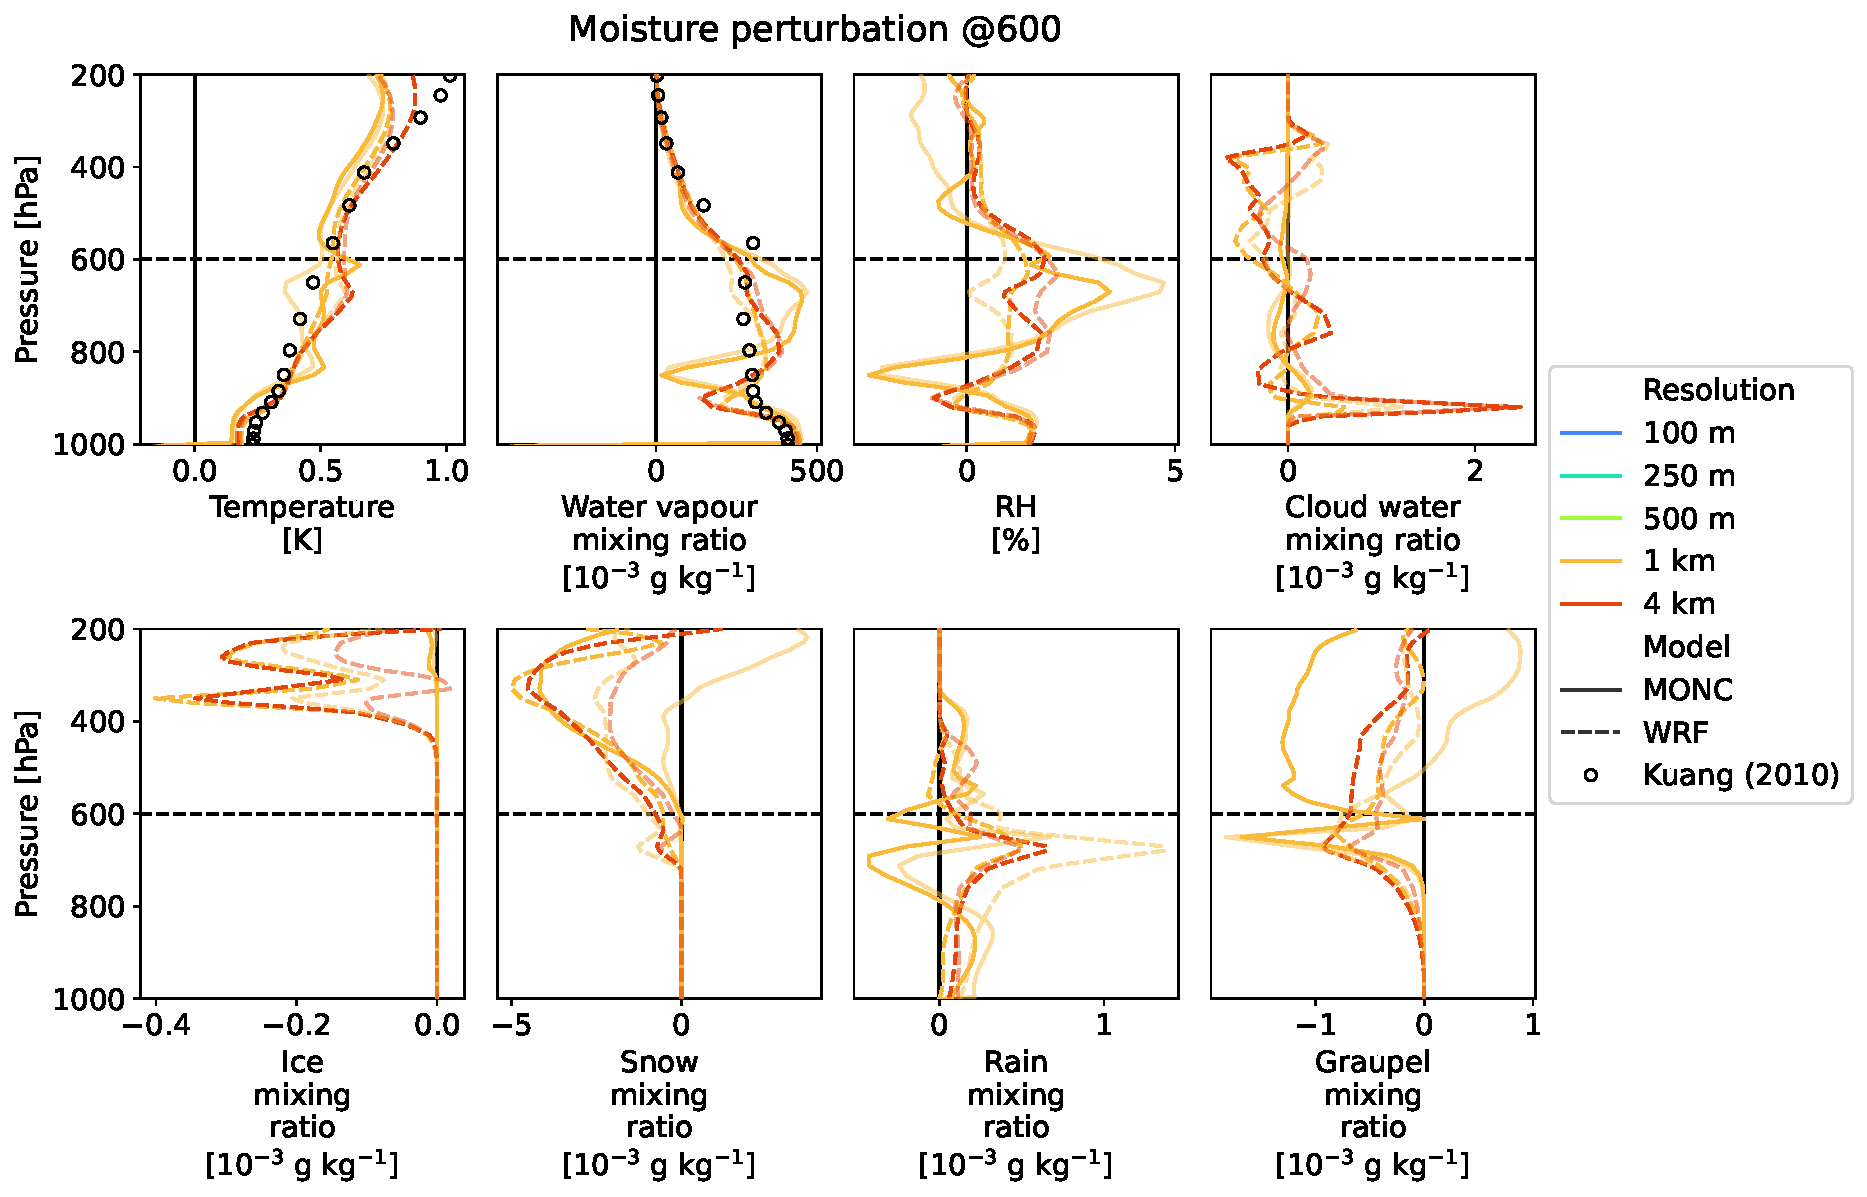
\includegraphics[width=\textwidth]{figures/pert_diffs_q_0.0002_@600}
    \caption{As in Figure \ref{fig:qpert_412}, but for a perturbation at 600
    hPa, and with black circles showing the responses of \citeA{Kuang_JAS_2010}
    to a specific humidity perturbation at 565 hPa.}
    \label{fig:qpert_600}
\end{figure}

\begin{figure}[pth]
    \noindent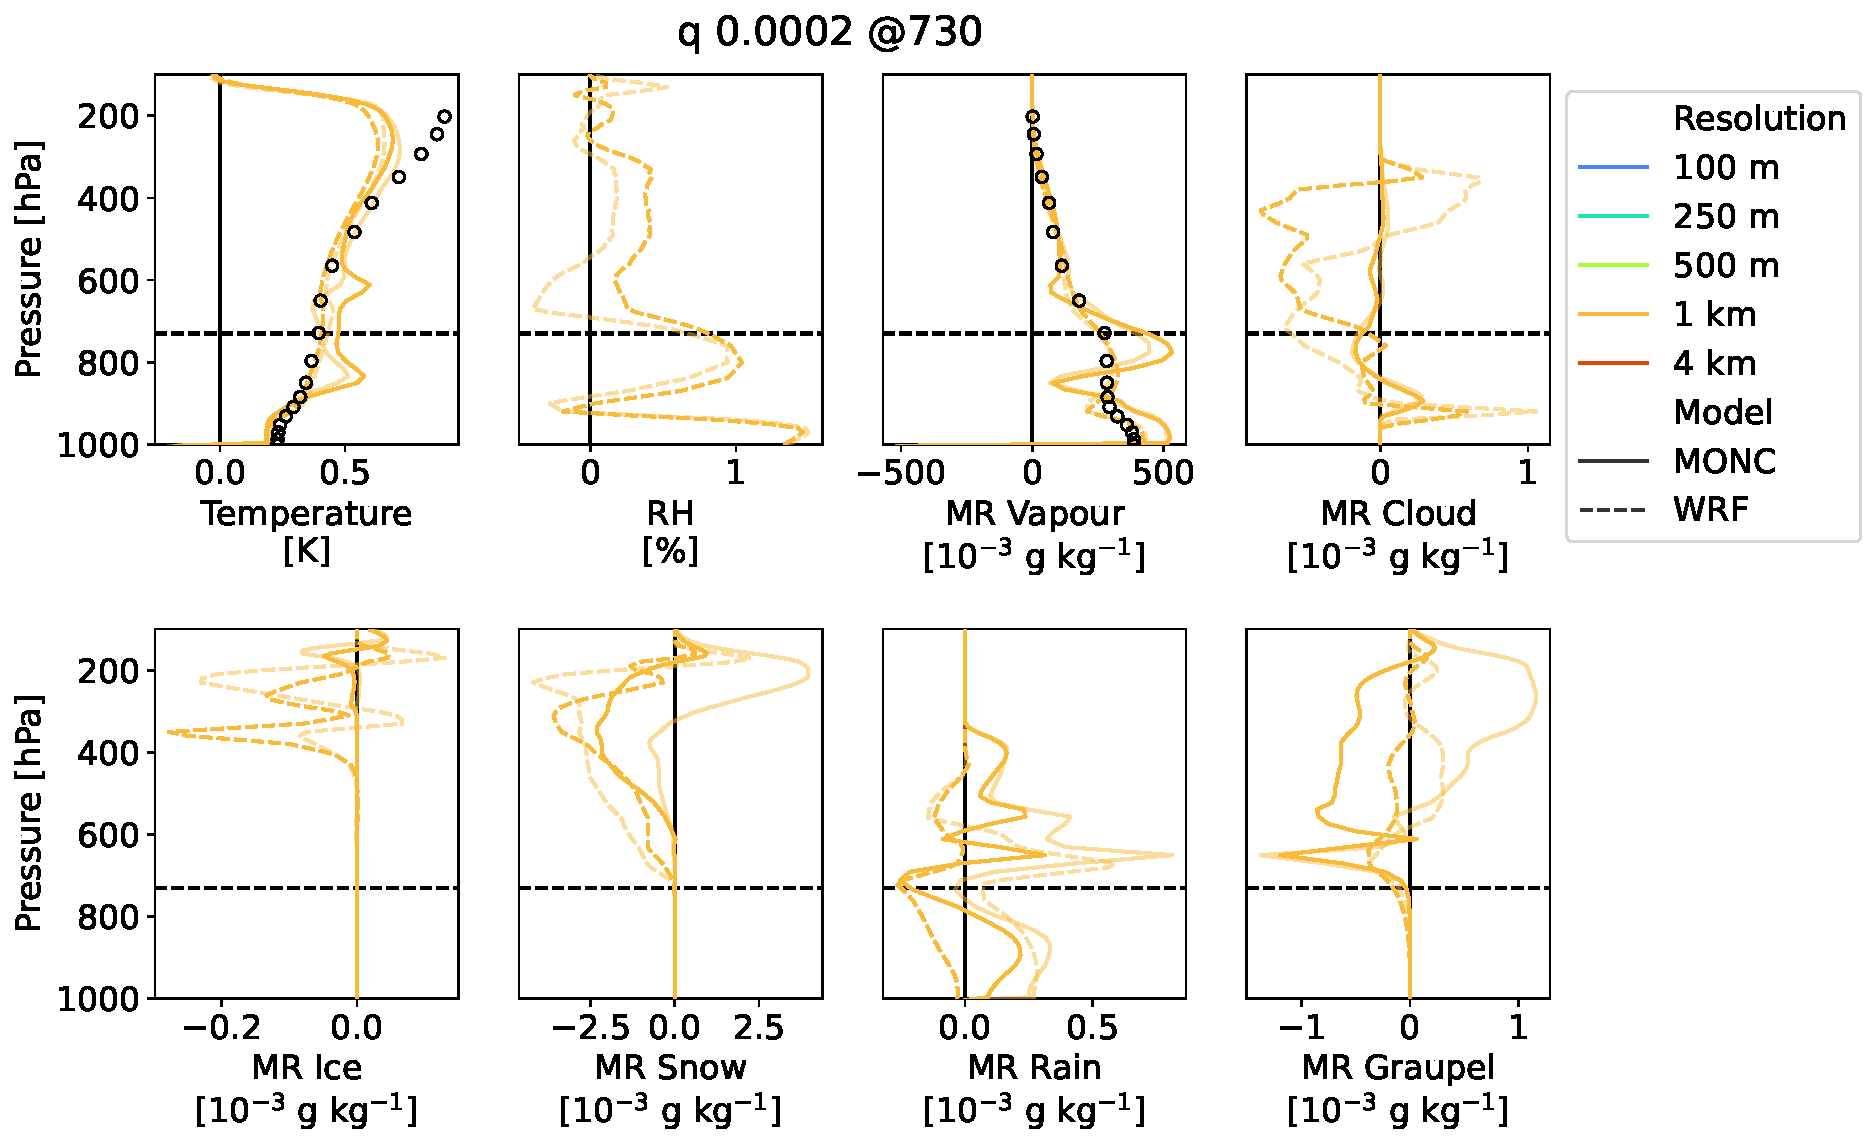
\includegraphics[width=\textwidth]{figures/pert_diffs_q_0.0002_@730}
    \caption{As in Figure \ref{fig:qpert_412}, but for a perturbation at 730
    hPa, and with black circles showing the responses of \citeA{Kuang_JAS_2010}
    to a specific humidity perturbation at 729 hPa.}
    \label{fig:qpert_730}
\end{figure}

\begin{figure}[pth]
    \noindent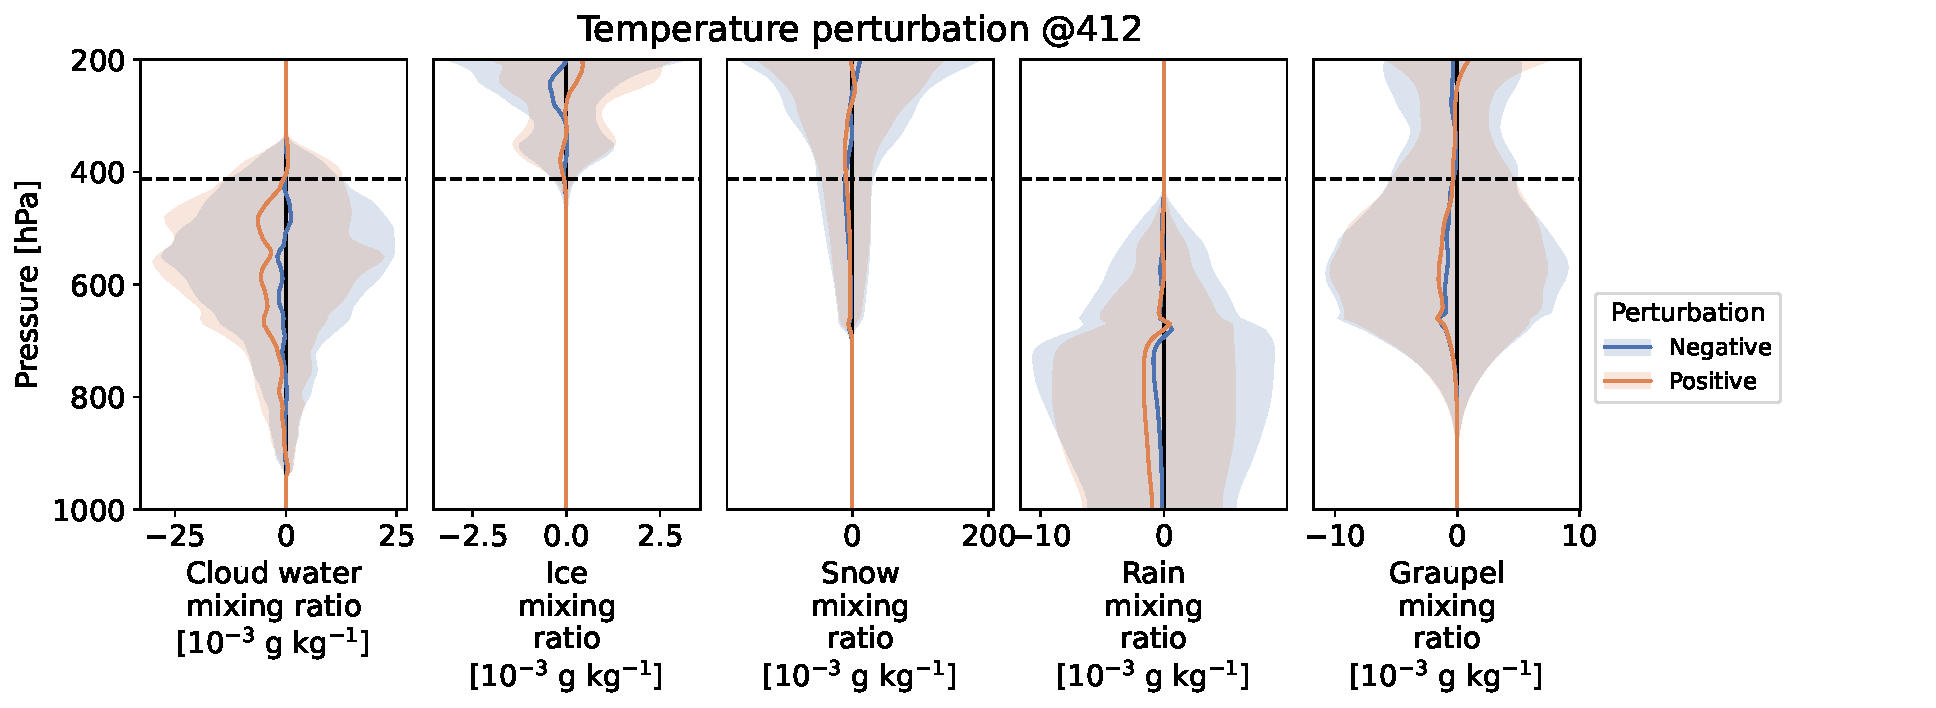
\includegraphics[width=\textwidth]{figures/pert_var_T_0.5_@412}
    \caption{Mean responses (solid line) and the $\pm$ 1 standard deviation
    range (shaded) for a temperature perturbation of $\pm$0.5 K at 412 hPa in
    the WRF runs at 100 m grid spacing. The solid vertical line shows zero
    response, the dashed horizontal line shows the level of maximum
    perturbation.}
    \label{fig:var_T_412}
\end{figure}

\begin{figure}[pth]
    \noindent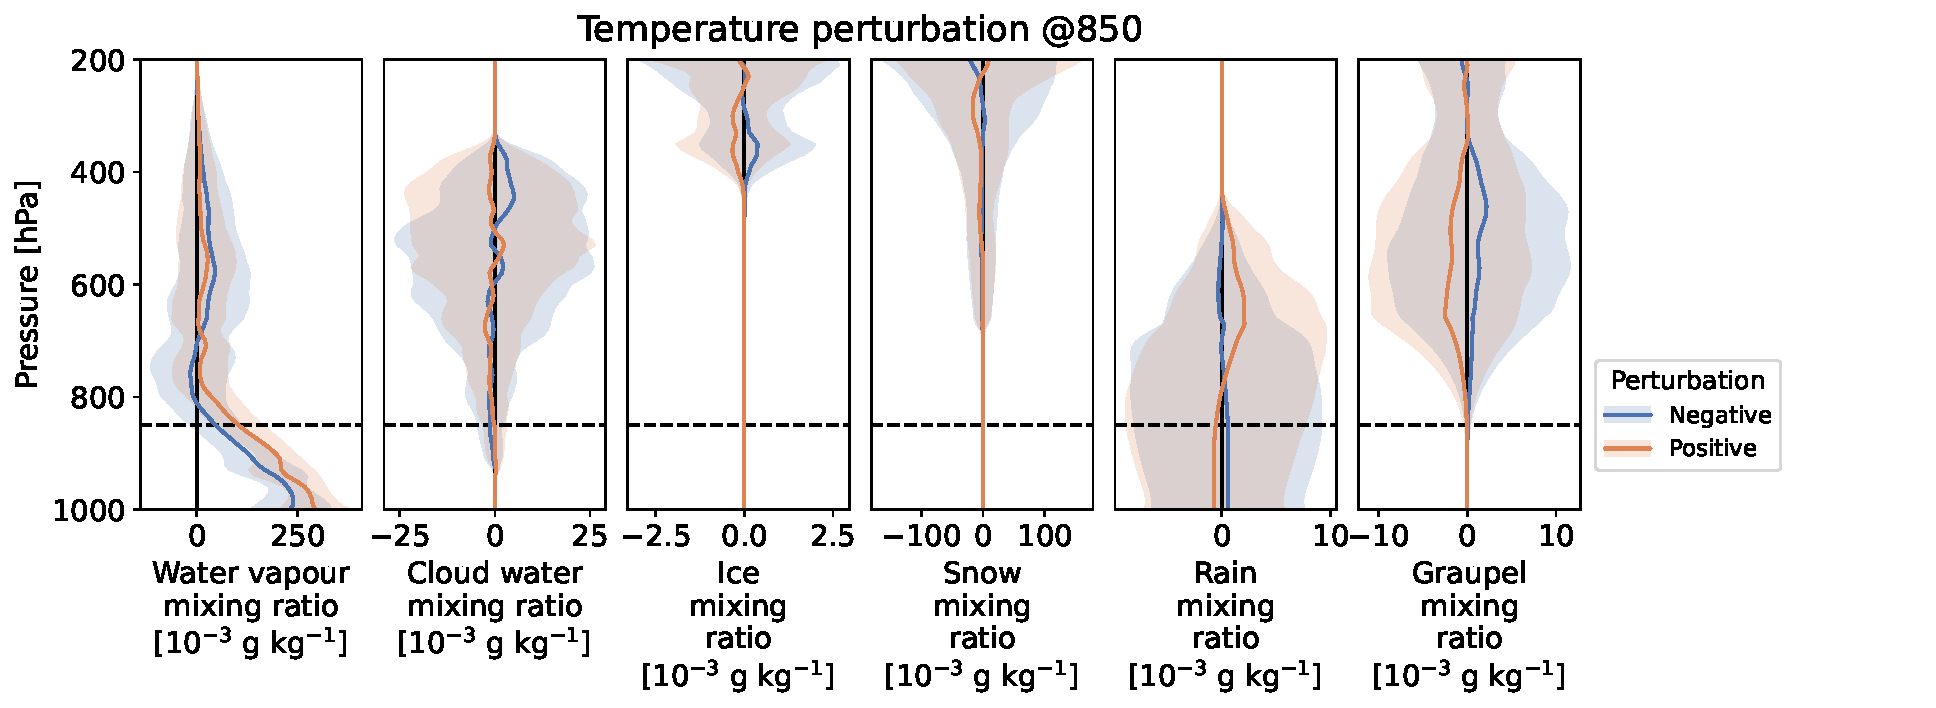
\includegraphics[width=\textwidth]{figures/pert_var_T_0.5_@850}
    \caption{As in Figure \ref{fig:var_T_412} but for a temperature perturbation
    at 850 hPa.}
    \label{fig:var_T_850}
\end{figure}

\begin{figure}[pth]
    \noindent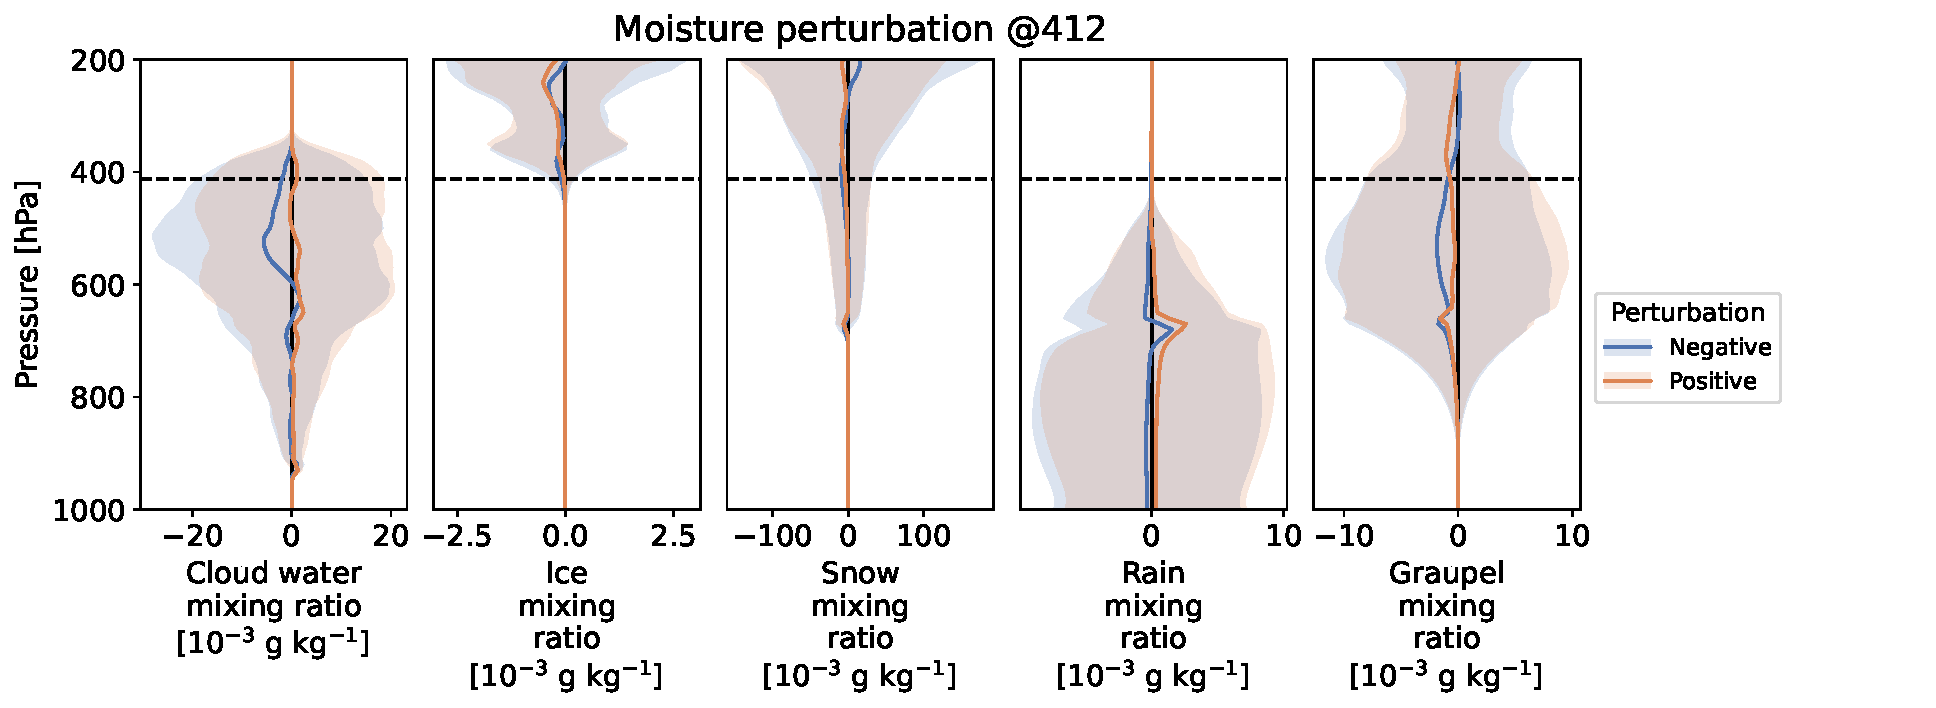
\includegraphics[width=\textwidth]{figures/pert_var_q_0.0002_@412}
    \caption{As in Figure \ref{fig:var_T_412} but for a water vapor mixing ratio
    perturbation of 0.2 g kg$^{-1}$ at 412 hPa.}
    \label{fig:var_q_412}
\end{figure}

\begin{figure}[pth]
    \noindent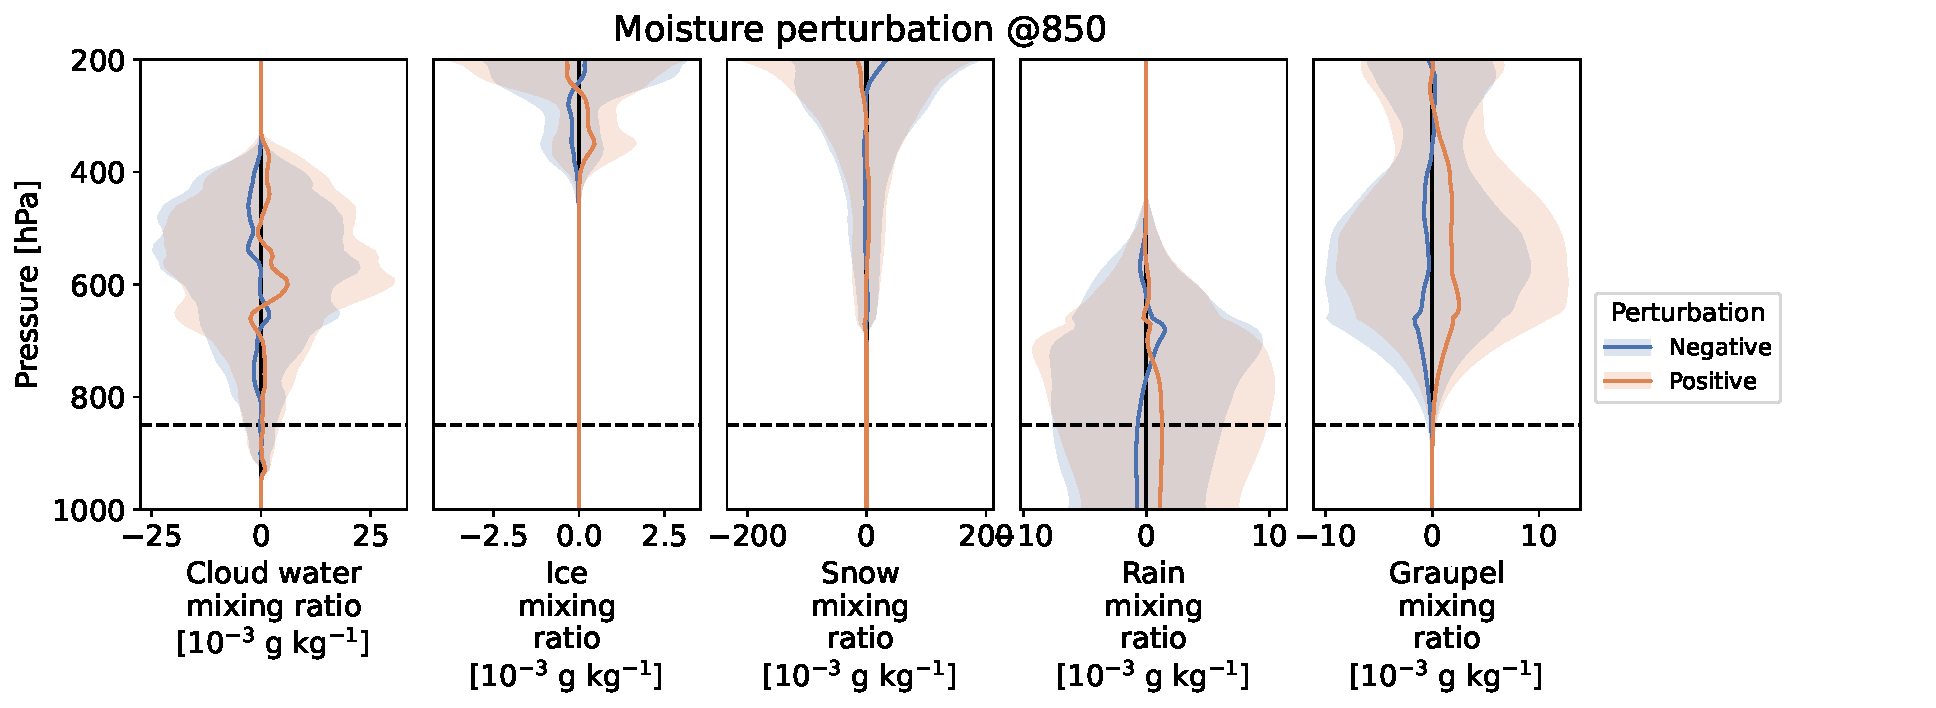
\includegraphics[width=\textwidth]{figures/pert_var_q_0.0002_@850}
    \caption{As in Figure \ref{fig:var_q_412} but for a water vapor mixing ratio
    perturbation of 0.2 g kg$^{-1}$ at 850 hPa.}
    \label{fig:var_q_850}
\end{figure}

\end{document}